% \documentclass[]{article}
% \documentclass[onecolumn]{IEEEtran}
% onecolumn for readability
\documentclass[]{IEEEtran}

% -----------------------------------------------------
% Preamble
% -----------------------------------------------------
% Math Packages
\usepackage{physics}
\usepackage{amsmath, amssymb, empheq}
\usepackage{thmtools}
% \usepackage[per-mode=symbol]{siunitx}

% Format Packages/Settings
\usepackage{todonotes}
\usepackage{xcolor}
\usepackage[]{hyperref}
\renewcommand{\figureautorefname}{Fig.}
% \usepackage[inline, shortlabels]{enumitem}
\usepackage{paralist}
\usepackage{cite}


% Theorems
\newtheorem{definition}{Definition}
\newtheorem{theorem}{Theorem}
\newtheorem{lemma}{Lemma}
\newtheorem{corollary}{Corollary}
\newtheorem{remark}{Remark}
\newtheorem{system}{System}

% % Custom Commands
\newcommand{\R}{\mathbb{R}}
% \newcommand{\N}{\mathbb{N}}
\newcommand{\st}{ \ | \ }

% \newcommand{\E}{\mathcal{E}}
% \newcommand{\Ebar}{\bar{\mathcal{E}}}
% \newcommand{\X}{\mathcal{X}}
% \newcommand{\Xbar}{\bar{\mathcal{X}}}
% % \newcommand{\U}{\mathcal{U}}
% % \newcommand{\Ubar}{\bar{\mathcal{U}}}
% \newcommand{\F}{\mathcal{F}}


%% Title and stuff
\title{
    MECH 6V29 - MPC - HW 4
}
\author{Jonas Wagner} % assuming Jonas and Justin... add Tanner?


% -----------------------------------------------------
% Begin Document
% -----------------------------------------------------
\begin{document}

% -----------------------------------------------------
% Title and Abstract
% -----------------------------------------------------
\maketitle
\begin{abstract}
    In this homework assignment an active suspension system was analyzed and controlled using both an LQR and an MPC controller.    
\end{abstract}


% -----------------------------------------------------
% Problem Definition
% -----------------------------------------------------
\section{Problem Definition}
The system to be controlled was provided in the MATLAB file as 
\begin{equation}
    \centering
    \begin{aligned}
        \dot{x}(t) &= \vb{A}_c x(t) + \vb{B}_c u(t) + \vb{V}_c d(t)\\
        y(t) &= \vb{C} x(t) + \vb{D} u(t) + \vb{W} d(t)
    \end{aligned}
\end{equation}
with states $x= \smqty[x_1 & x_2 & x_3 & x_4]^T \in \R^{n_x=4}$ (tire-deflection, unsprung mass velocity, suspension deflection, and sprung mass velocity), input $u = u_1 \in \R^{n_u=1}$ (active suspension force), disturbances $d = \smqty[d_1 & d_2]^T \in \R^{n_d=2}$ (road height change and road height), and outputs $y = \smqty[y_1 & y_2 & y_3]^T \in \R^{n_y=3}$ (unsprung mass height, sprung mass height, and spring mass acceleration).
The matrices are defined as 
\begin{gather*}
    \vb{A}_c = \mqty[
        0 & 1 & 0 & 0\\
        -\frac{K_t}{M_u} & -\frac{B_s + B_t}{M_u} & \frac{K_s}{M_u} & \frac{B_s}{M_u}\\
        0 & -1 & 0 & 1\\
        0 & \frac{B_s}{M_s} & -\frac{K_s}{M_s} & -\frac{B_s}{M_s}
        ]
    \vb{B}_c = \mqty[0\\ \frac{-1}{M_u}\\ 0 \\ \frac{1}{M_s}]
    \\
    C = \mqty[
        1 & 0 & 0 & 0\\
        1 & 0 & 1 & 0\\
        0 & \frac{B_s}{M_s} & -\frac{K_s}{M_s} & -\frac{B_s}{M_s}
    ]
    D = \mqty[0 \\ 0 \\ \frac{1}{M_s}]
    \\
    \vb{V}_c = \mqty[-1 & 0\\ 
        \frac{B_t}{M_u} & 0\\
        0 & 0\\
        0 & 0
    ]
    W = \mqty[0 & 1\\ 0 & 1 \\ 0 & 0]
\end{gather*}
with parameters $K_s = 900$ [N/m], $K_t = 2500$ [N/m], $M_s = 2.45$ [kg], $M_u = 1$ [kg], $B_s = 7.5$ [s/m], and $B_t = 5$ [s/m].

The code derives the DT-LTI system at different discretization time steps depending on the selected velocity and the disturbance data.

In addition, bounds on the states, inputs, and disturbances were provided as the intervals:
\begin{gather*}
    x \in \mathcal{X} = \qty{x\in \R^{n_x} \st \abs{x} \leq \mqty[0.01\\1\\0.03\\1]}
    \\
    u \in \mathcal{U} = \qty{u \in \R^{n_u} \st \abs{u} \leq 30}
    \\
    d \in \mathcal{D} = \qty{d \in \R^{n_d} \st \abs{d} \leq \mqty[0.5\\0.02]}
\end{gather*}


% -----------------------------------------------------
% Open Loop Dynamics
% -----------------------------------------------------
\section{Open-Loop Dynamics}
Initial open-loop dynamics are simulated with lsim() and the provided disturbance data resulting in the poor response dynamics shown in \autoref{fig:open-loop} for the realistic road profile (IRI\_737b) along with the synthetic roadBumpHole road profiles.
(See appendix for additional results)
From these dynamics the high oscillatory (and poor dampening) effects can easily be observed.
The first state, tire deflection ($x_1$), was often exceeding the acceptable state bounds.

\begin{figure}[h]
    \centering
    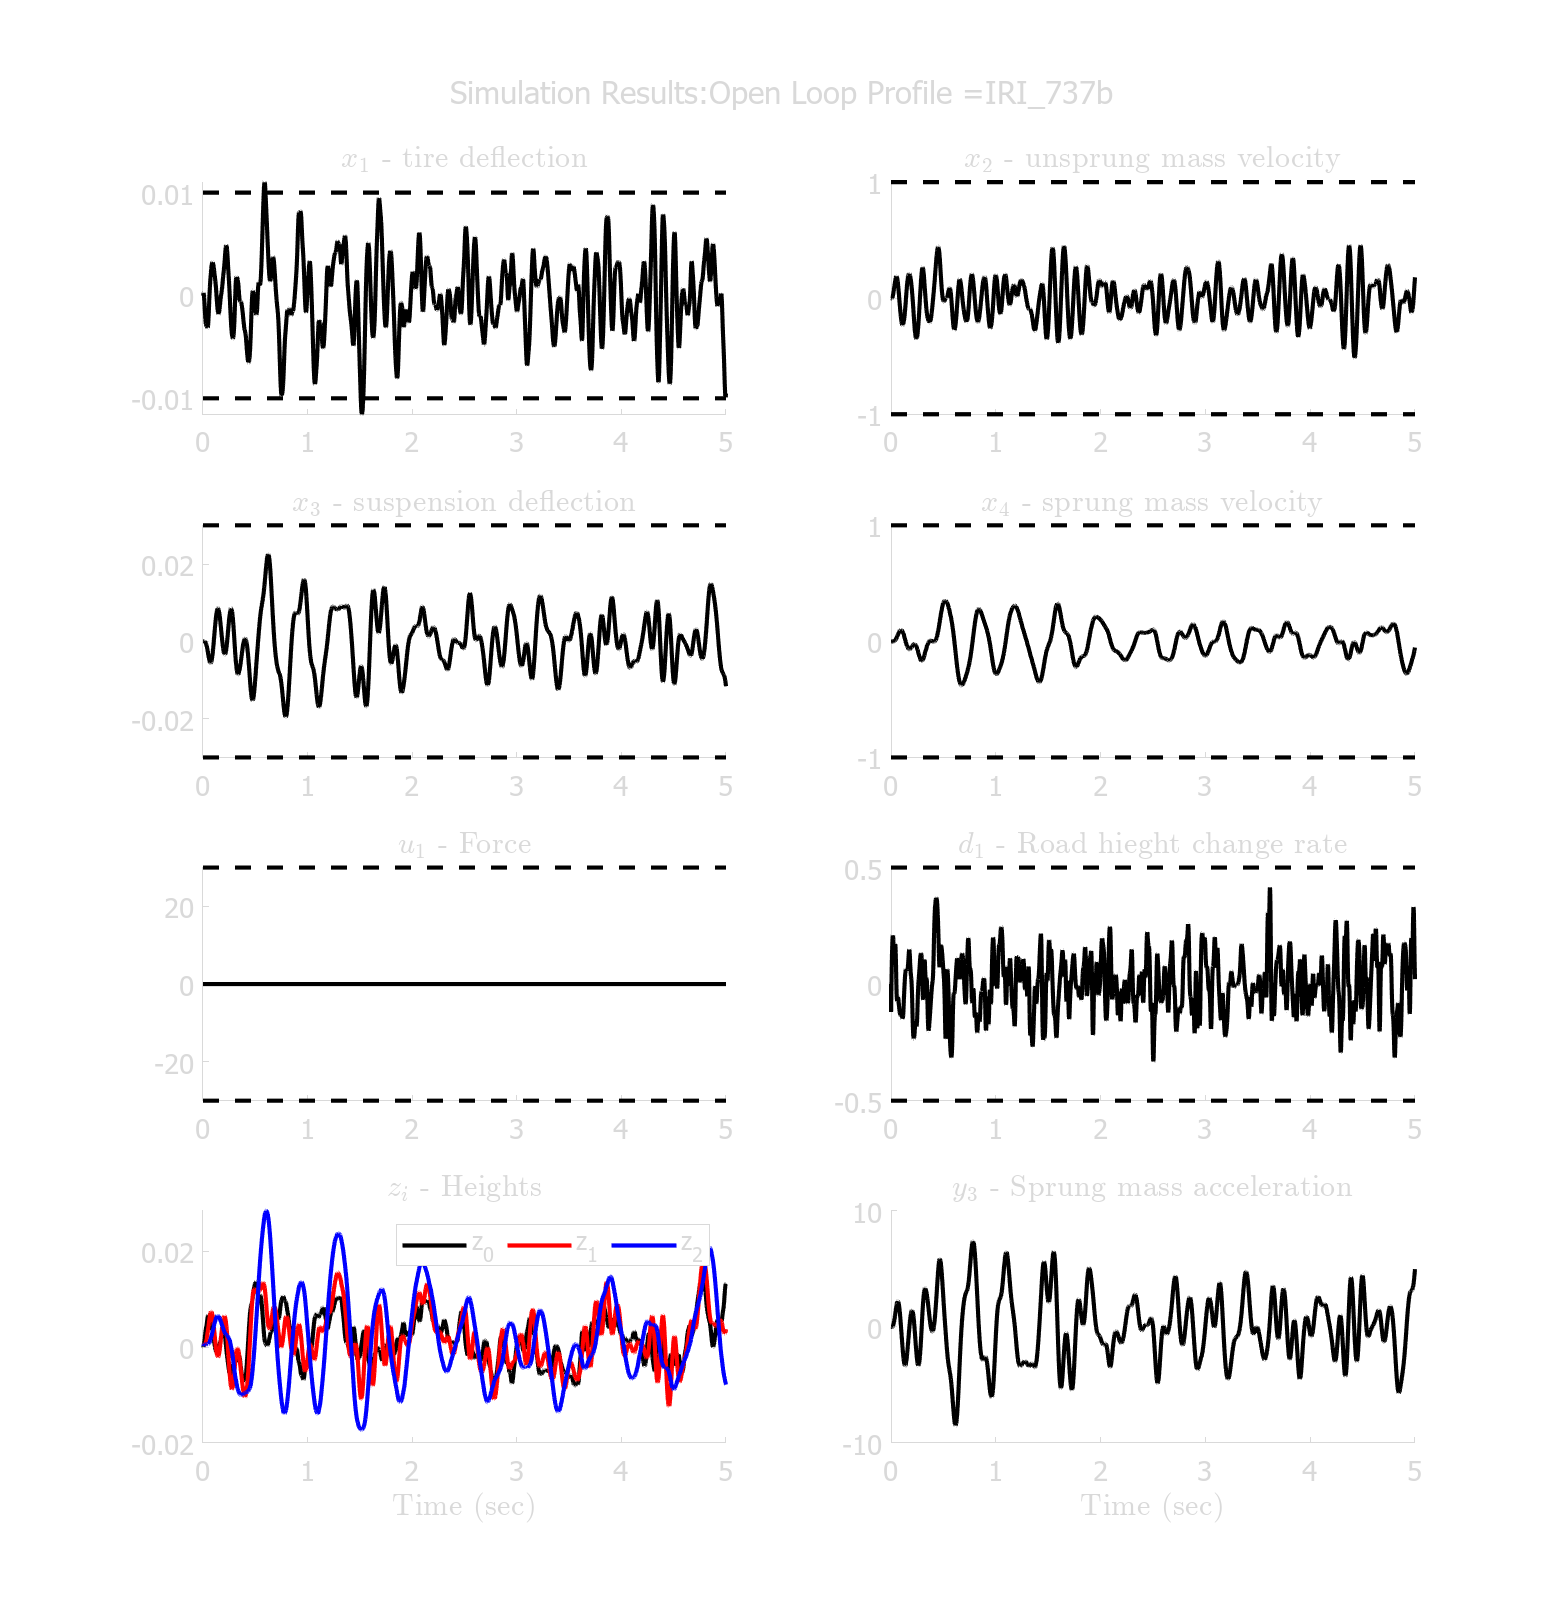
\includegraphics[width = 0.49 \columnwidth]{figs/results_open_IRI_737b.png}
    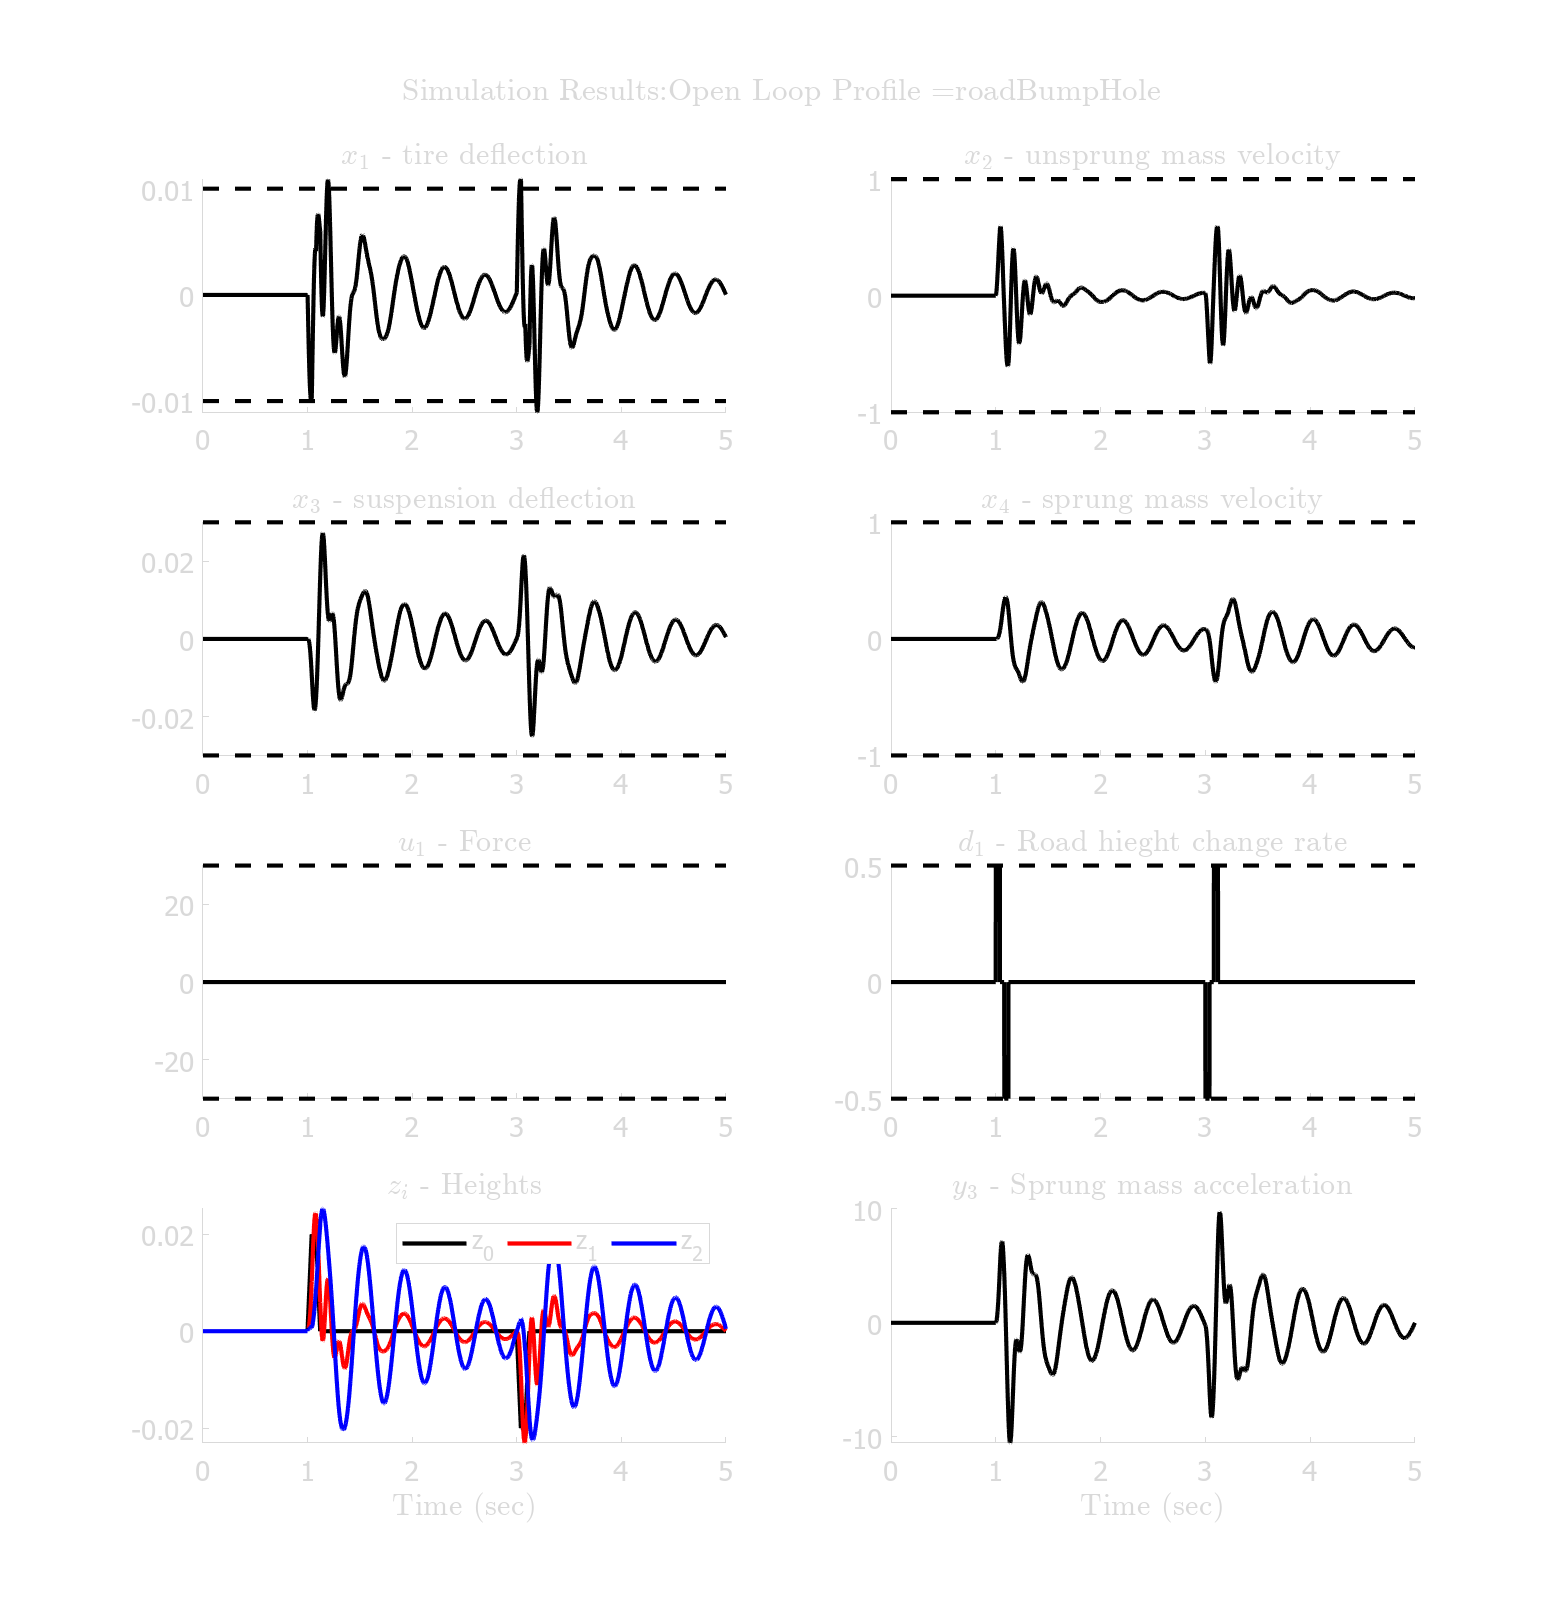
\includegraphics[width = 0.49 \columnwidth]{figs/results_open_roadBumpHole.png}
    % 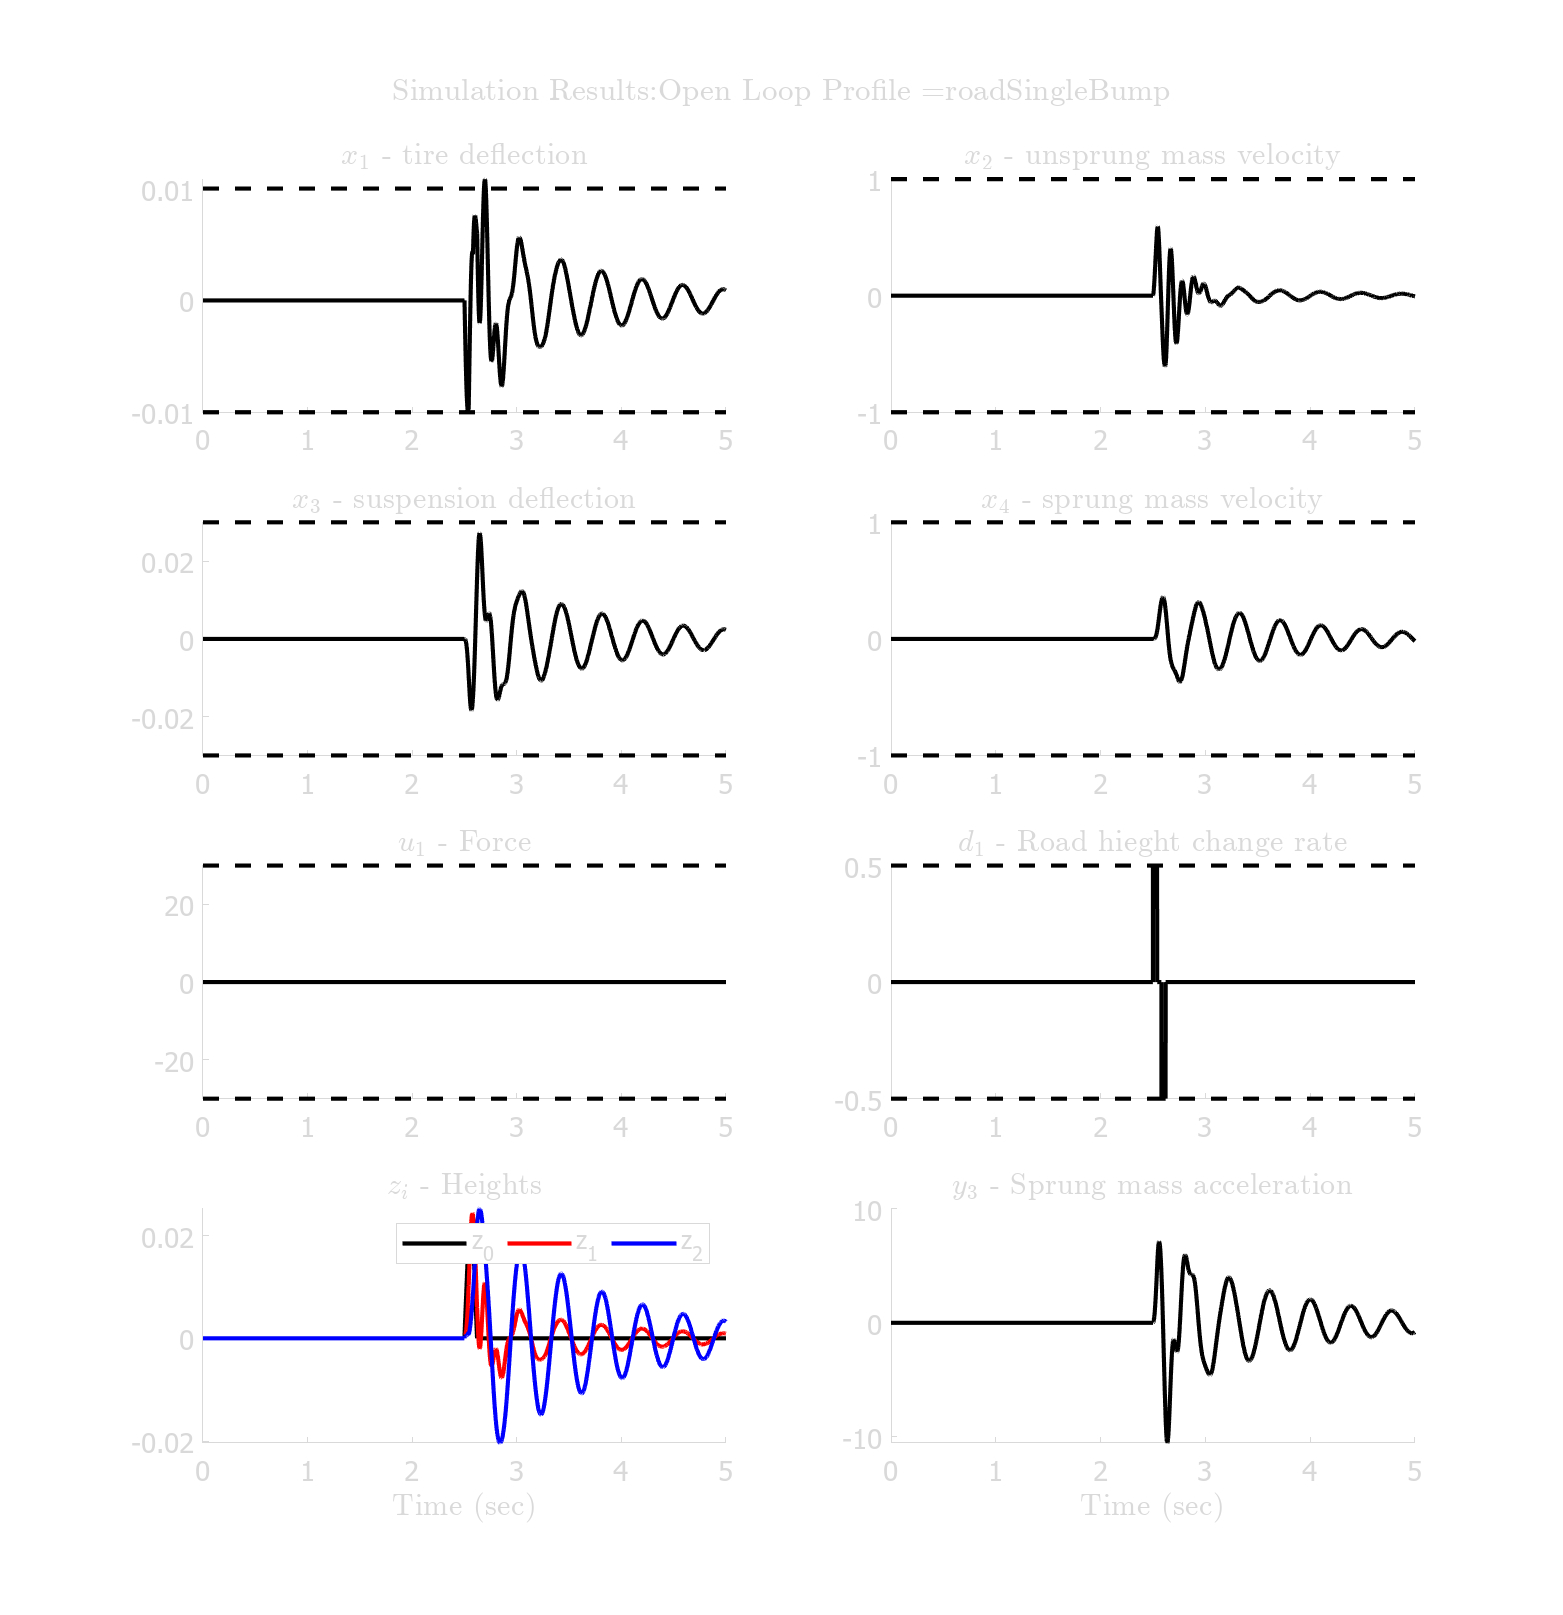
\includegraphics[width = 0.49 \columnwidth]{figs/results_open_roadSingleBump.png}
    % 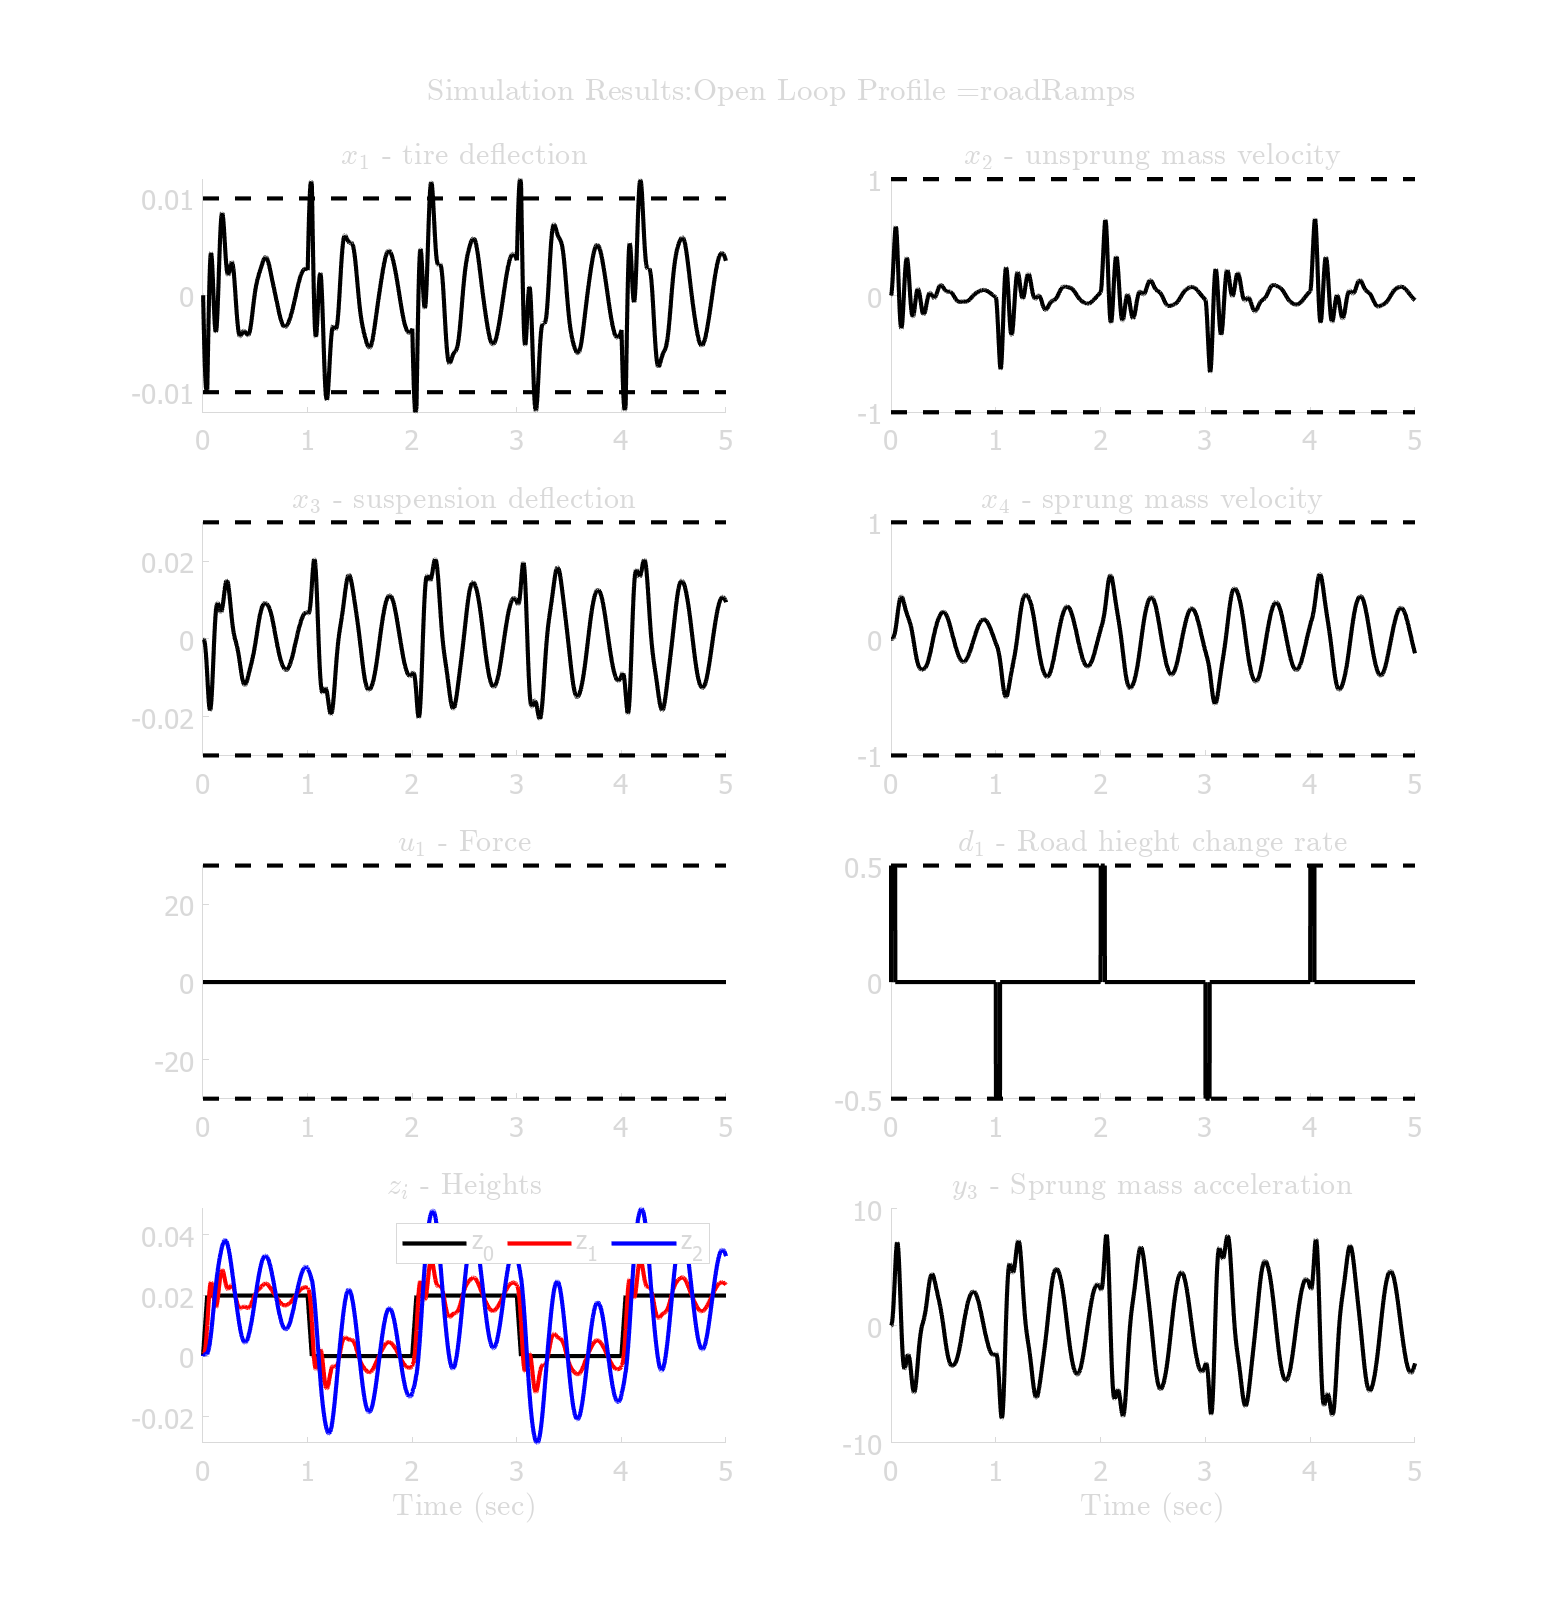
\includegraphics[width = 0.49 \columnwidth]{figs/results_open_roadRamps.png}
    \caption{Open-loop dynamics for the IRI\_737b  and roadBumpHole road profiles.} \label{fig:open-loop}
\end{figure}


% \newpage
% -----------------------------------------------------
% LQR Controller Design
% -----------------------------------------------------
\section{LQR Controller Design}
Initial LQR controller designs were implemented and tested to provide a baseline optimization function for the MPC controller itself.
The MATLAB lqr() function was used to design a controller with designed $Q$ and $R$ matrices.

Two primary cost matrices for state-optimization were developed: direct acceleration minimization ($Q_{accel}$) and bound-based optimization ($Q_{bounds}$).
\begin{align}
    Q_{accel} &= \frac{10^5}{\norm{C^T C}_\infty} \cdot C^T \smqty[\dmat{0,0,1}] C
    \\
    Q_{bounds} &= 10^3 \cdot \smqty[\dmat{\frac{1}{0.01},1,\frac{1}{0.03},1}]
\end{align}
These were tested individually and combined as $Q_{both} = Q_{accel} + Q_{bounds}$.

For the input cost, a simple inverse bound cost was used:
\begin{gather}
    R = \mqty[\dmat{\frac{1}{0.5}, \frac{1}{0.02}}]
\end{gather}

The simulations are provided in \autoref{fig:lqr_accel}, \autoref{fig:lqr_bounds}, and \autoref{fig:lqr_both} respectively.

\begin{figure}[h]
    \centering
    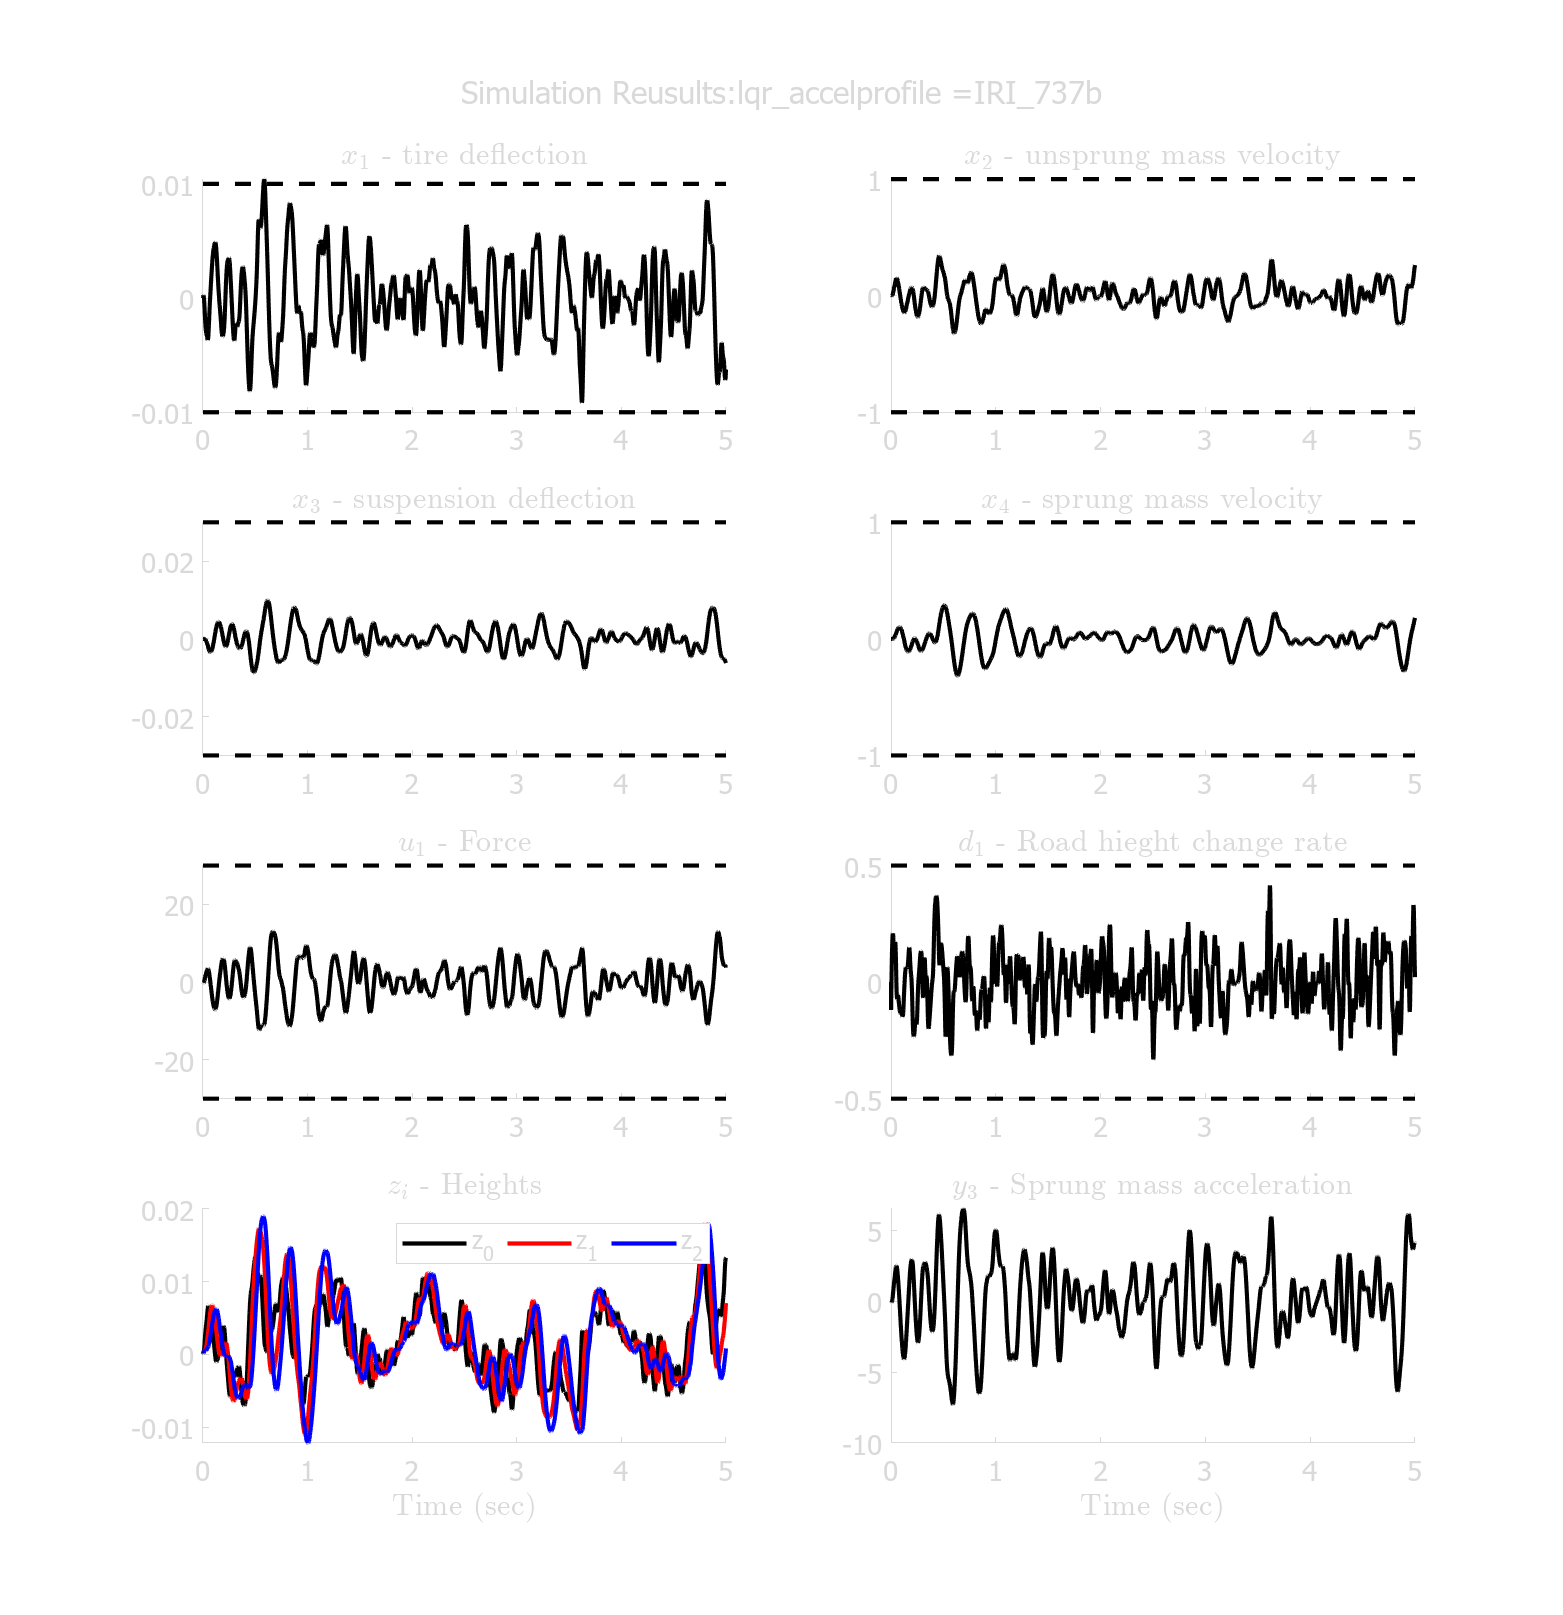
\includegraphics[width = 0.49 \columnwidth]{figs/results_lqr_accel_IRI_737b.png}
    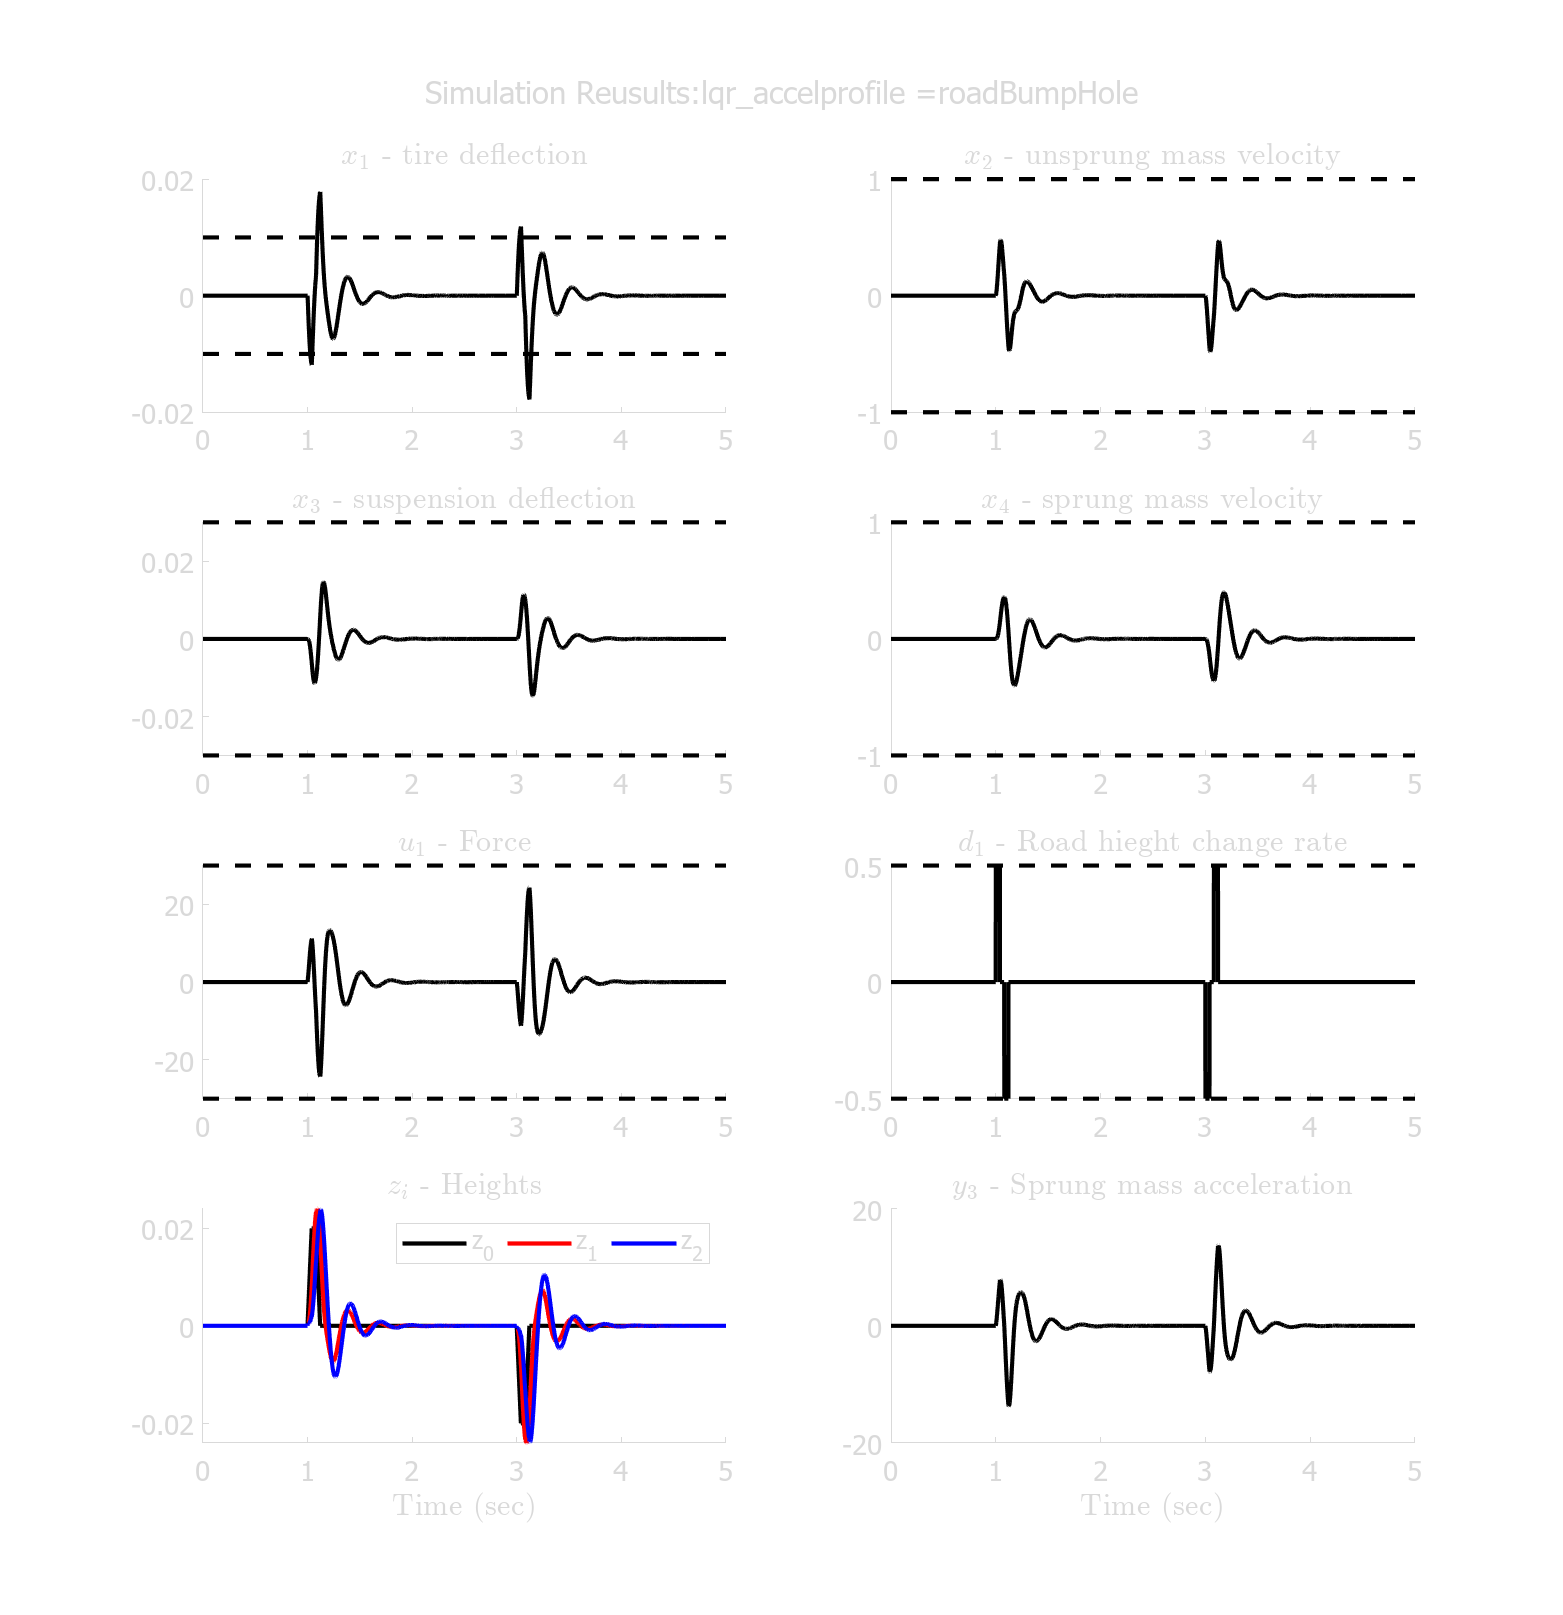
\includegraphics[width = 0.49 \columnwidth]{figs/results_lqr_accel_roadBumpHole.png}
    % 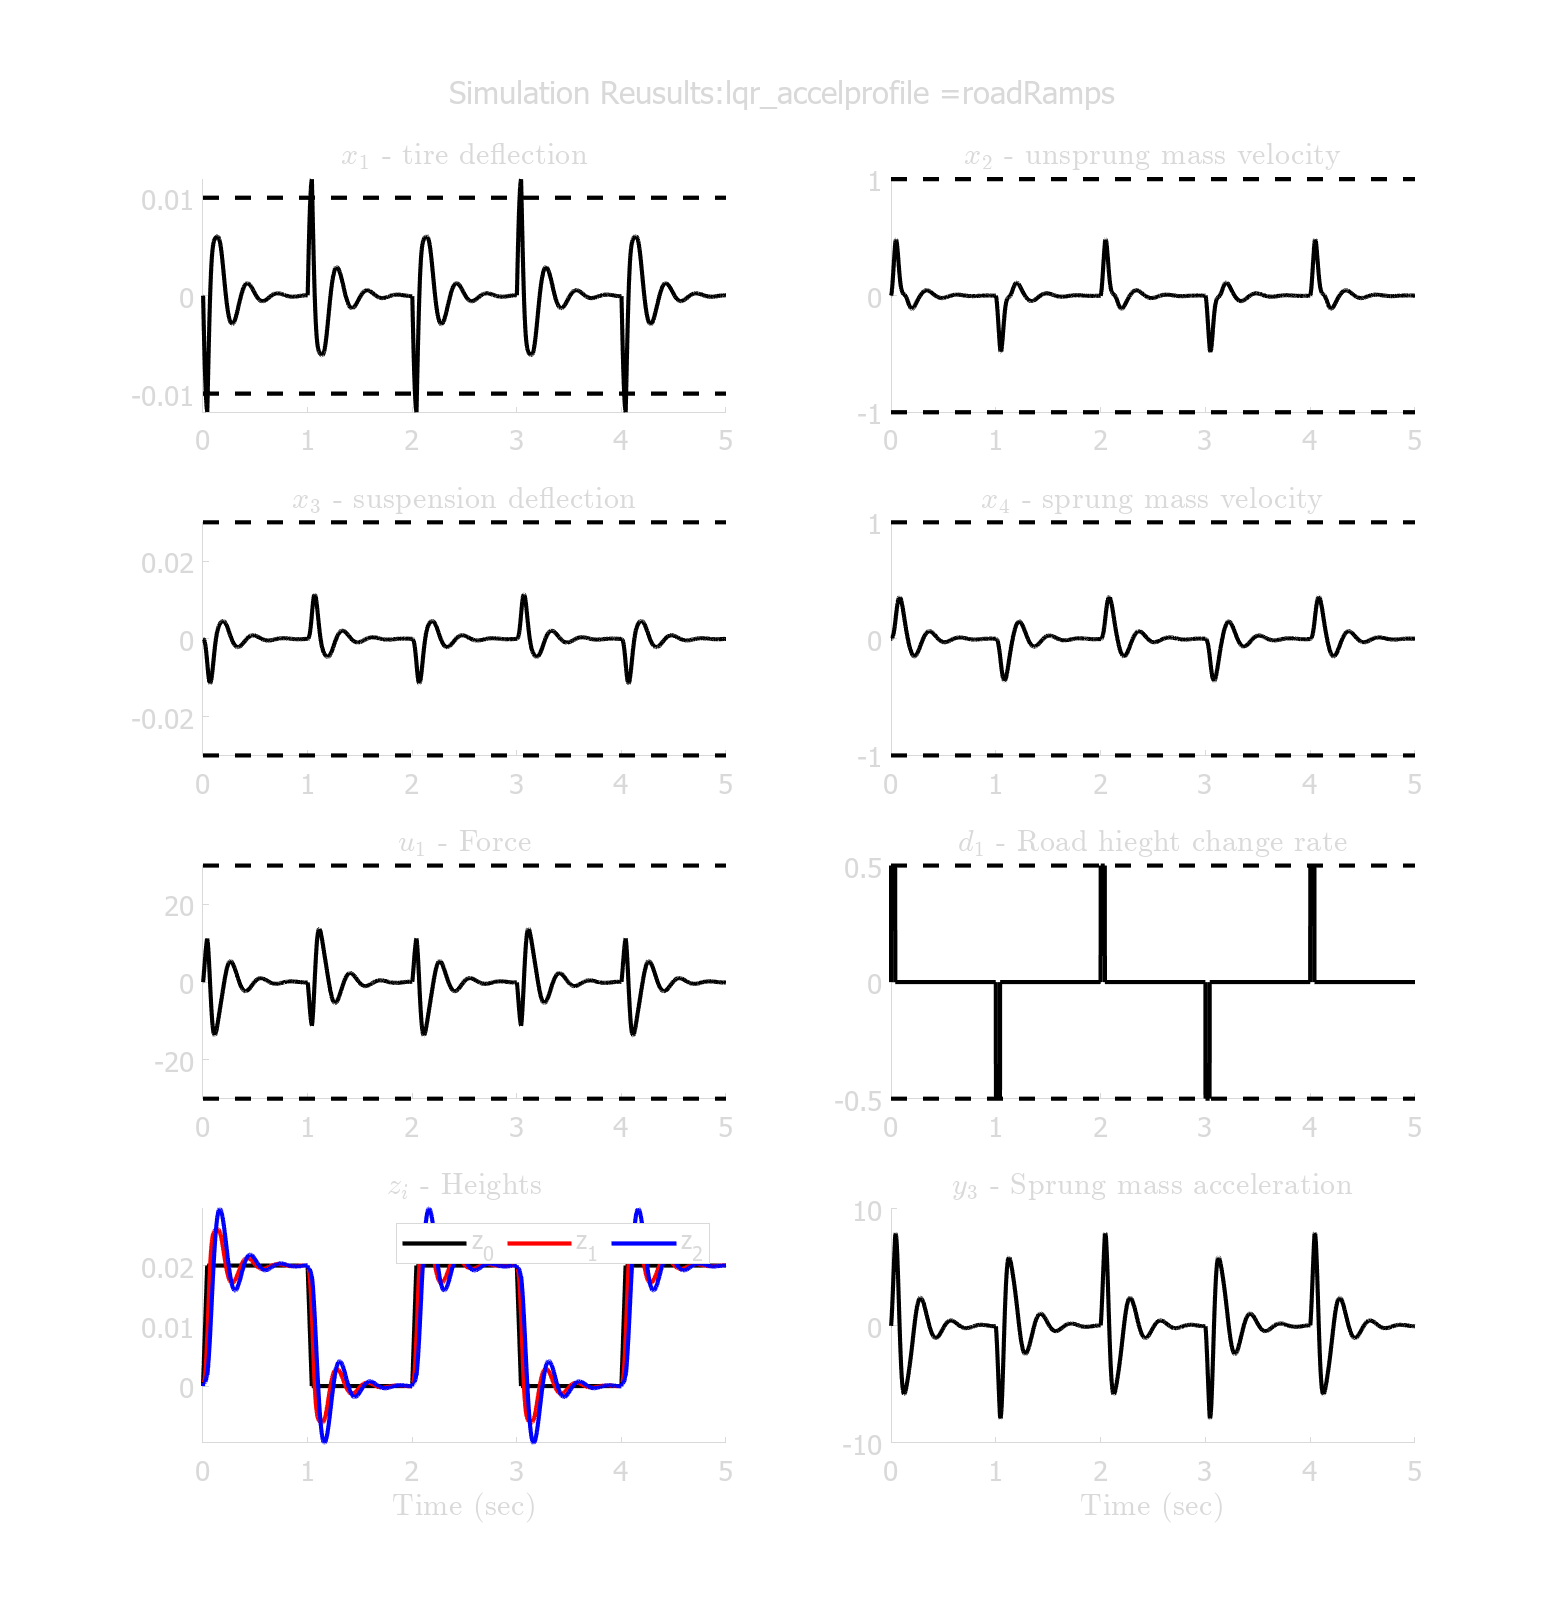
\includegraphics[width = 0.49 \columnwidth]{figs/results_lqr_accel_roadRamps.png}
    % 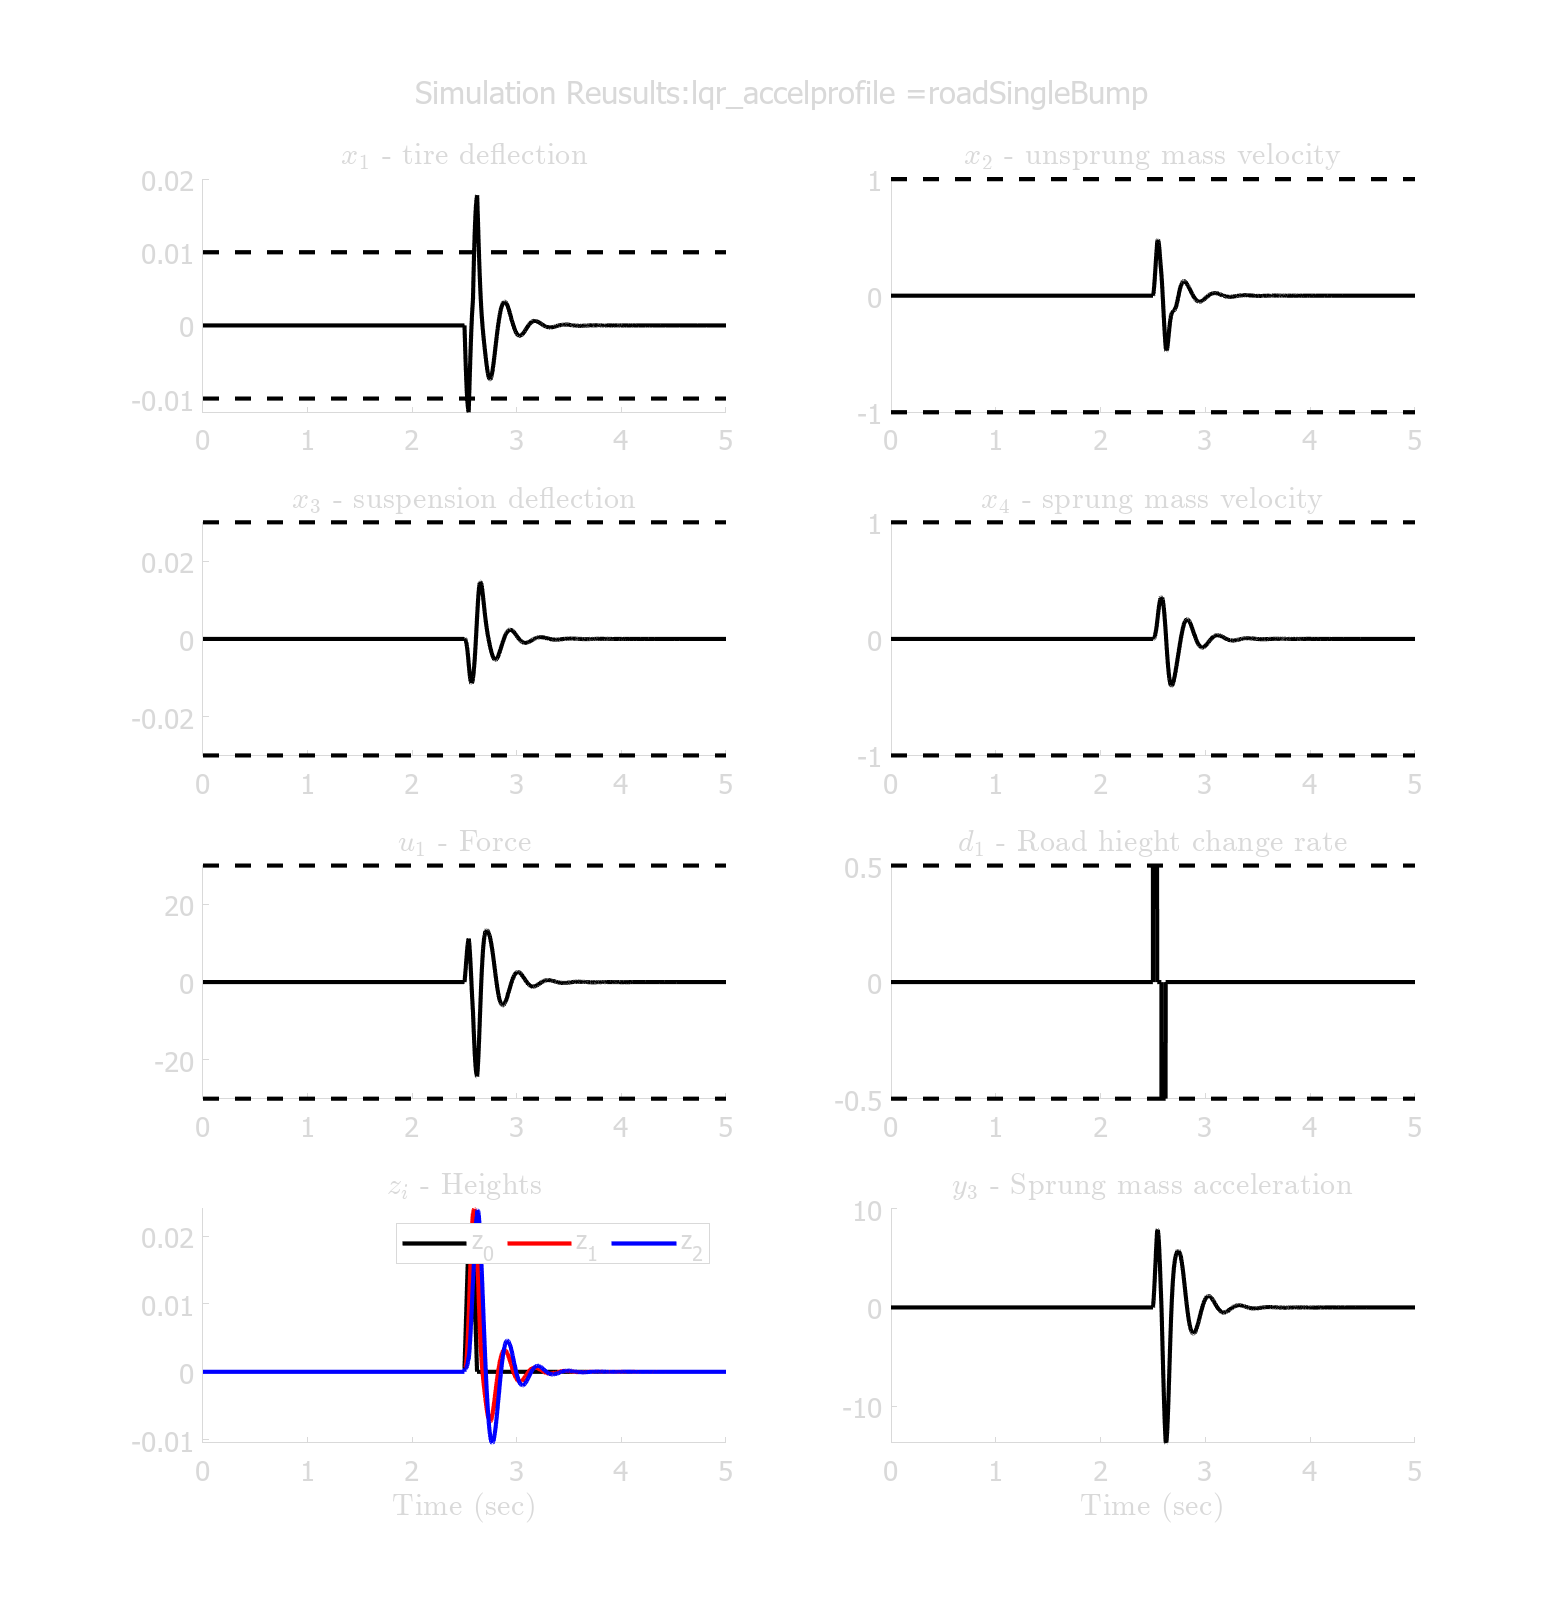
\includegraphics[width = 0.49 \columnwidth]{figs/results_lqr_accel_roadSingleBump.png}
    \caption{LQR closed-loop dynamics with $Q_{accel}$ and $R$ for the IRI\_737b  and roadBumpHole road profiles.} \label{fig:lqr_accel}
\end{figure}

\begin{figure}[h]
    \centering
    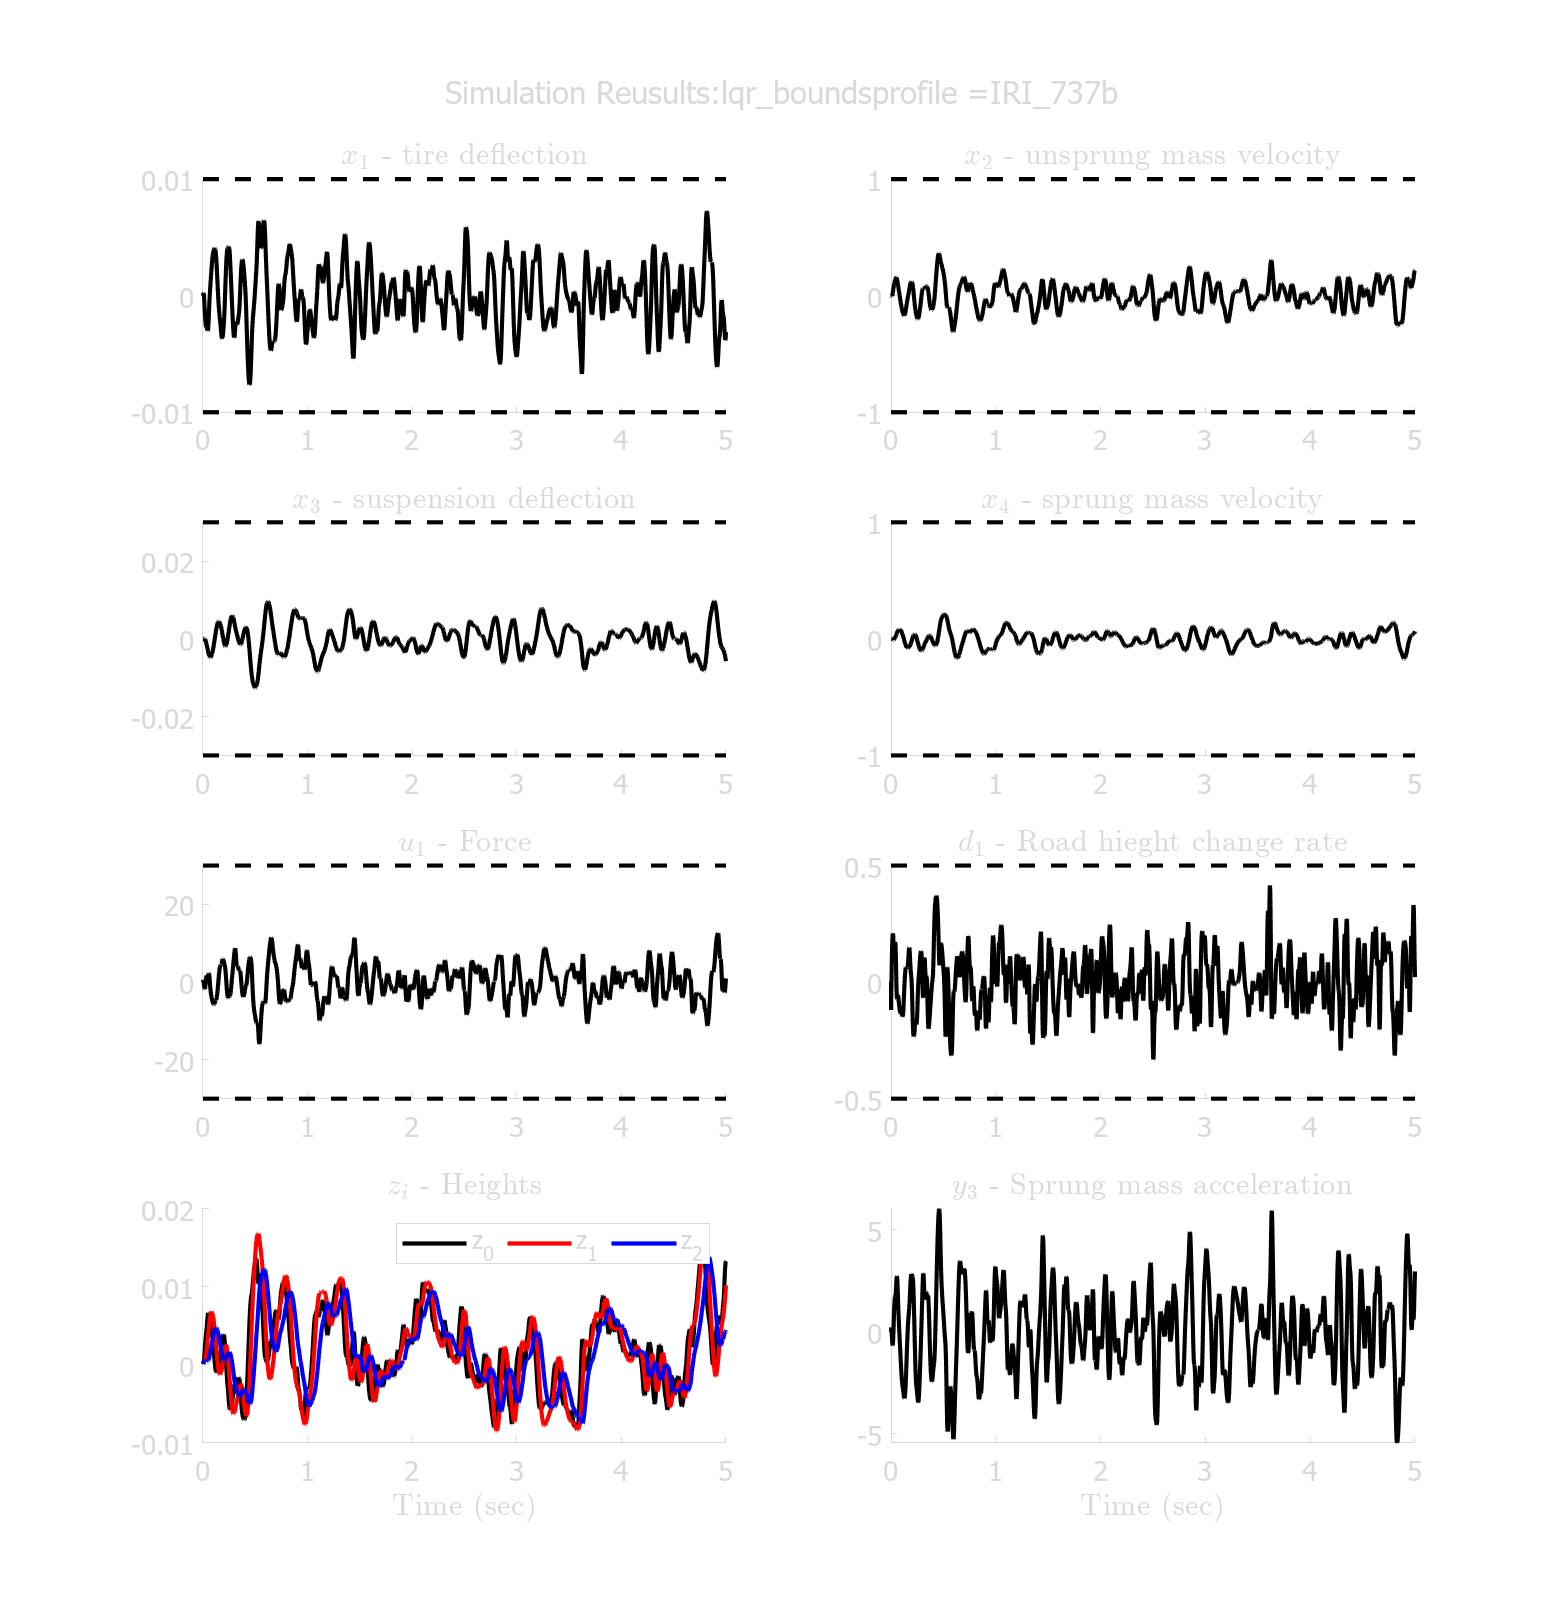
\includegraphics[width = 0.49 \columnwidth]{figs/results_lqr_bounds_IRI_737b.png}
    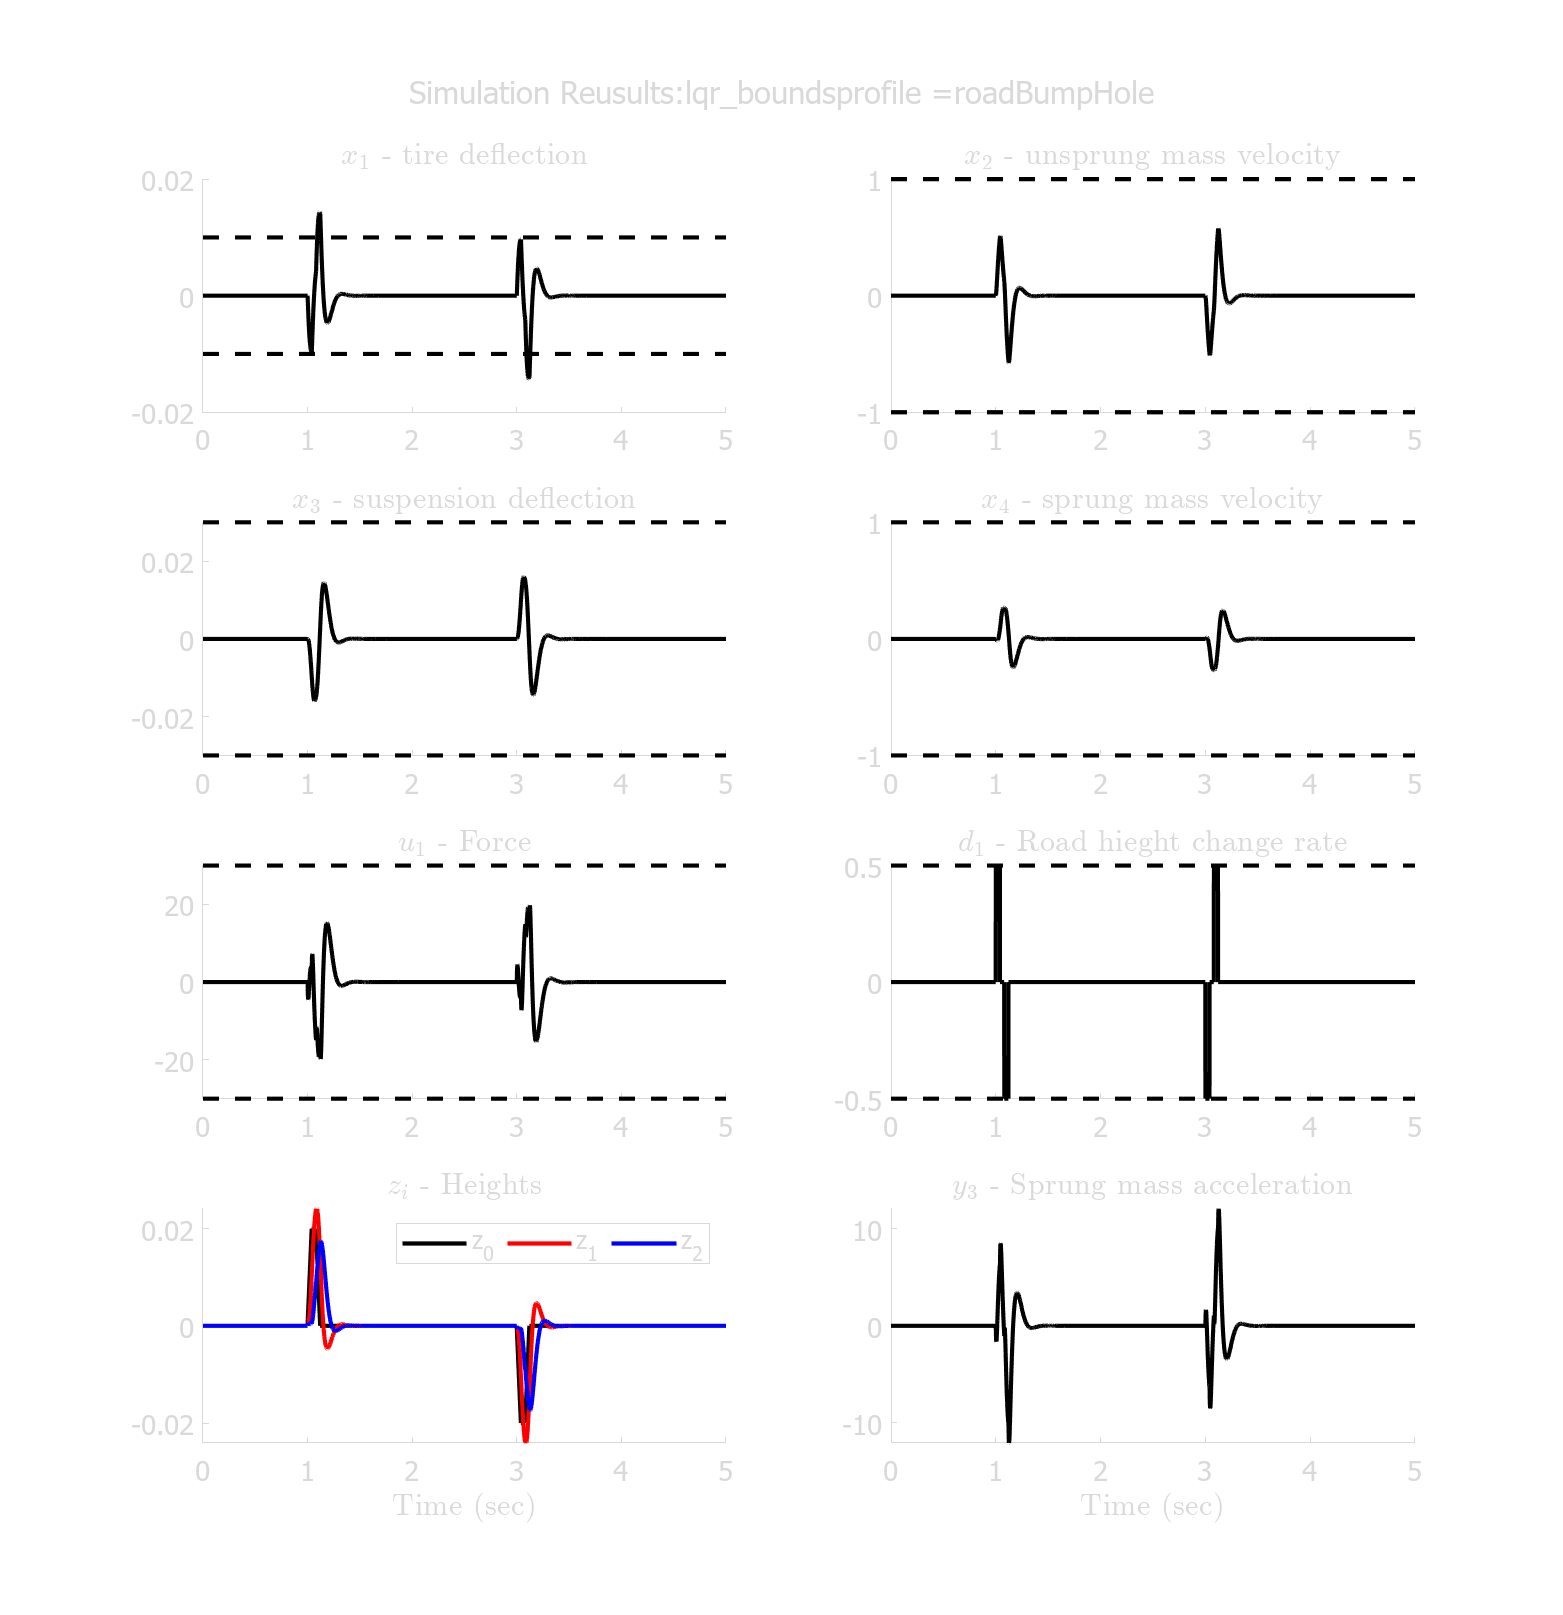
\includegraphics[width = 0.49 \columnwidth]{figs/results_lqr_bounds_roadBumpHole.png}
    % 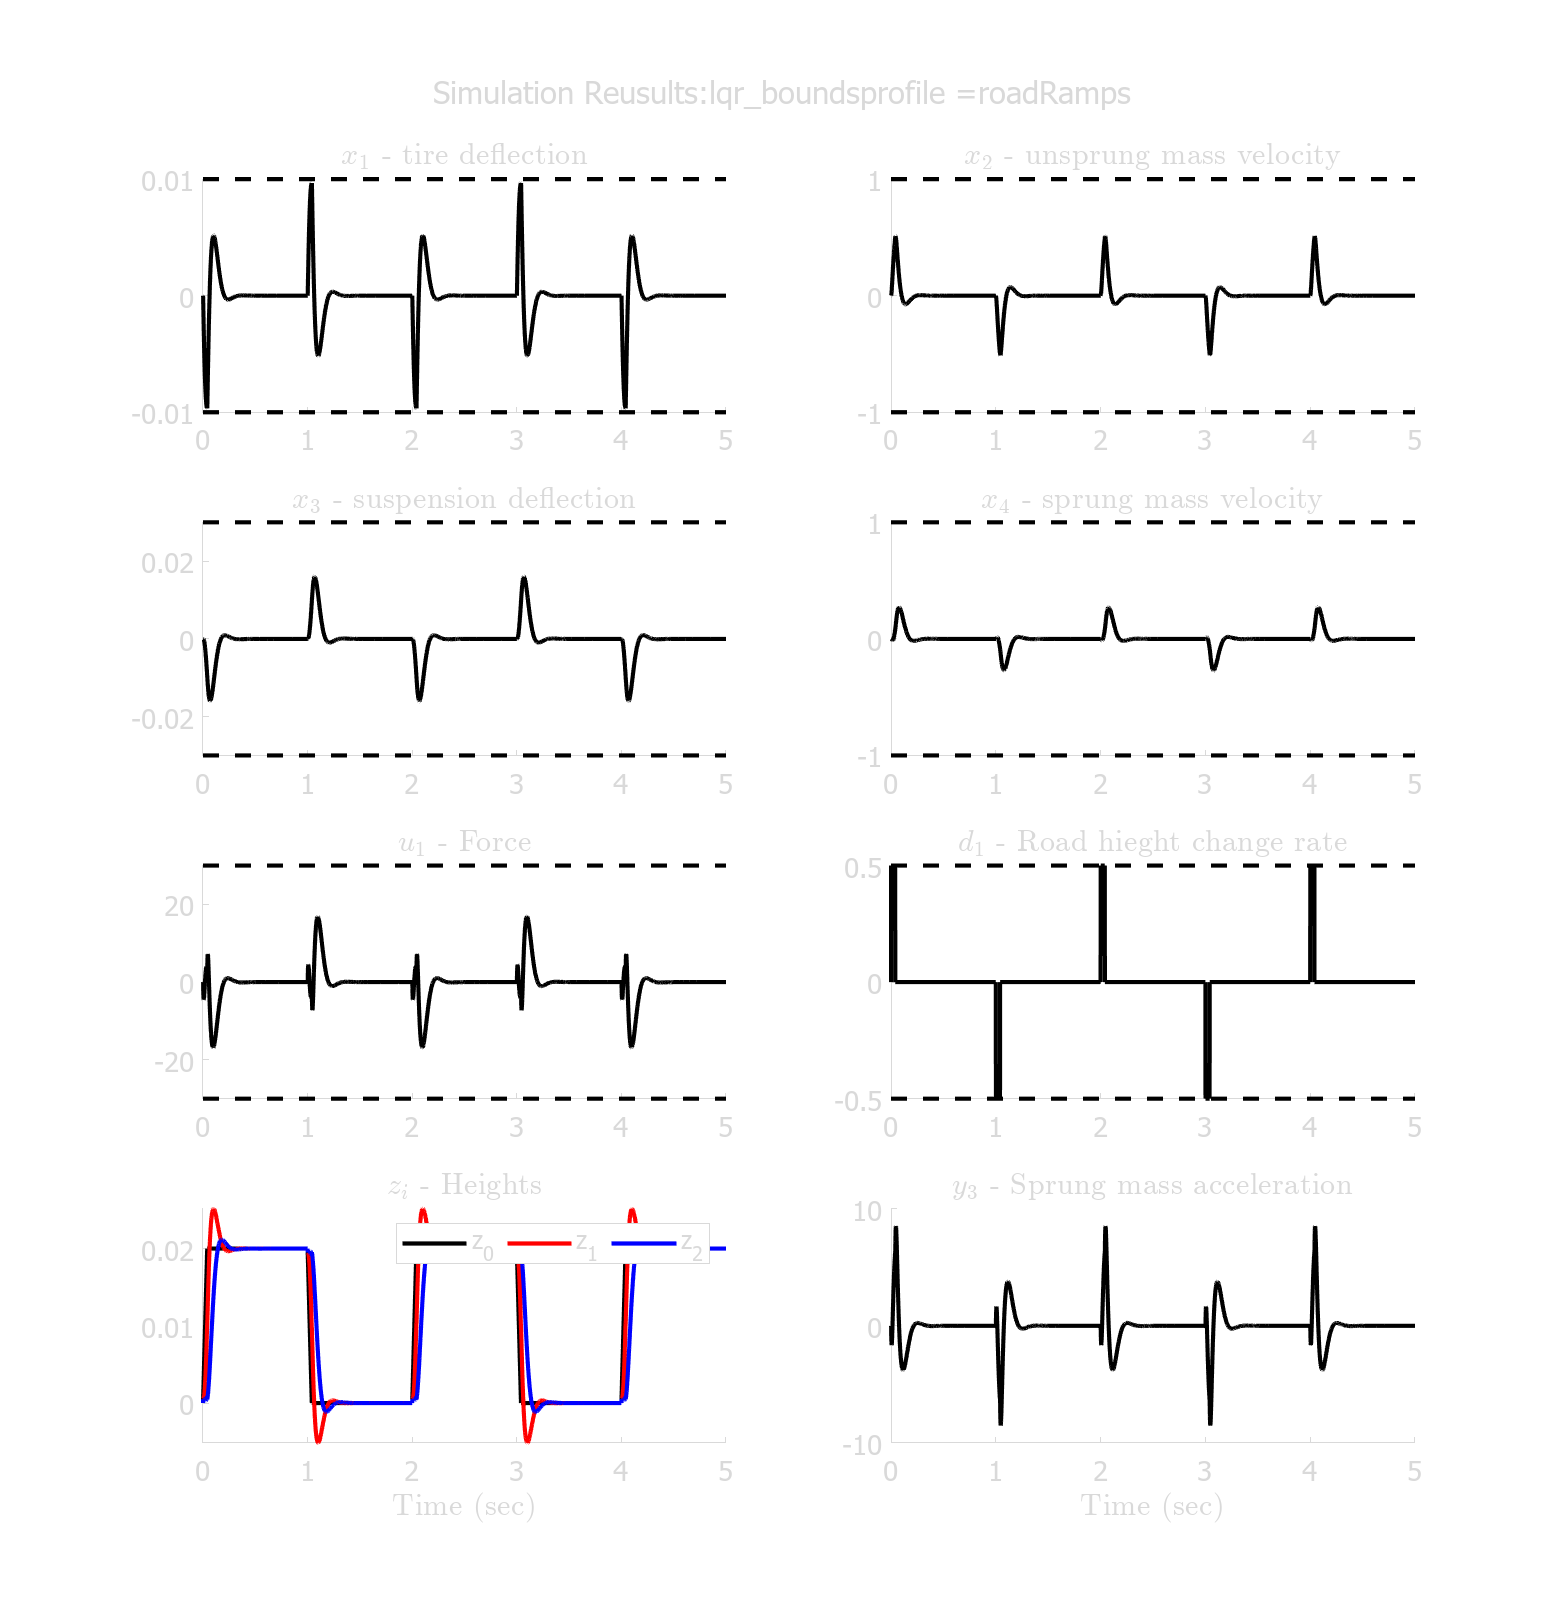
\includegraphics[width = 0.49 \columnwidth]{figs/results_lqr_bounds_roadRamps.png}
    % 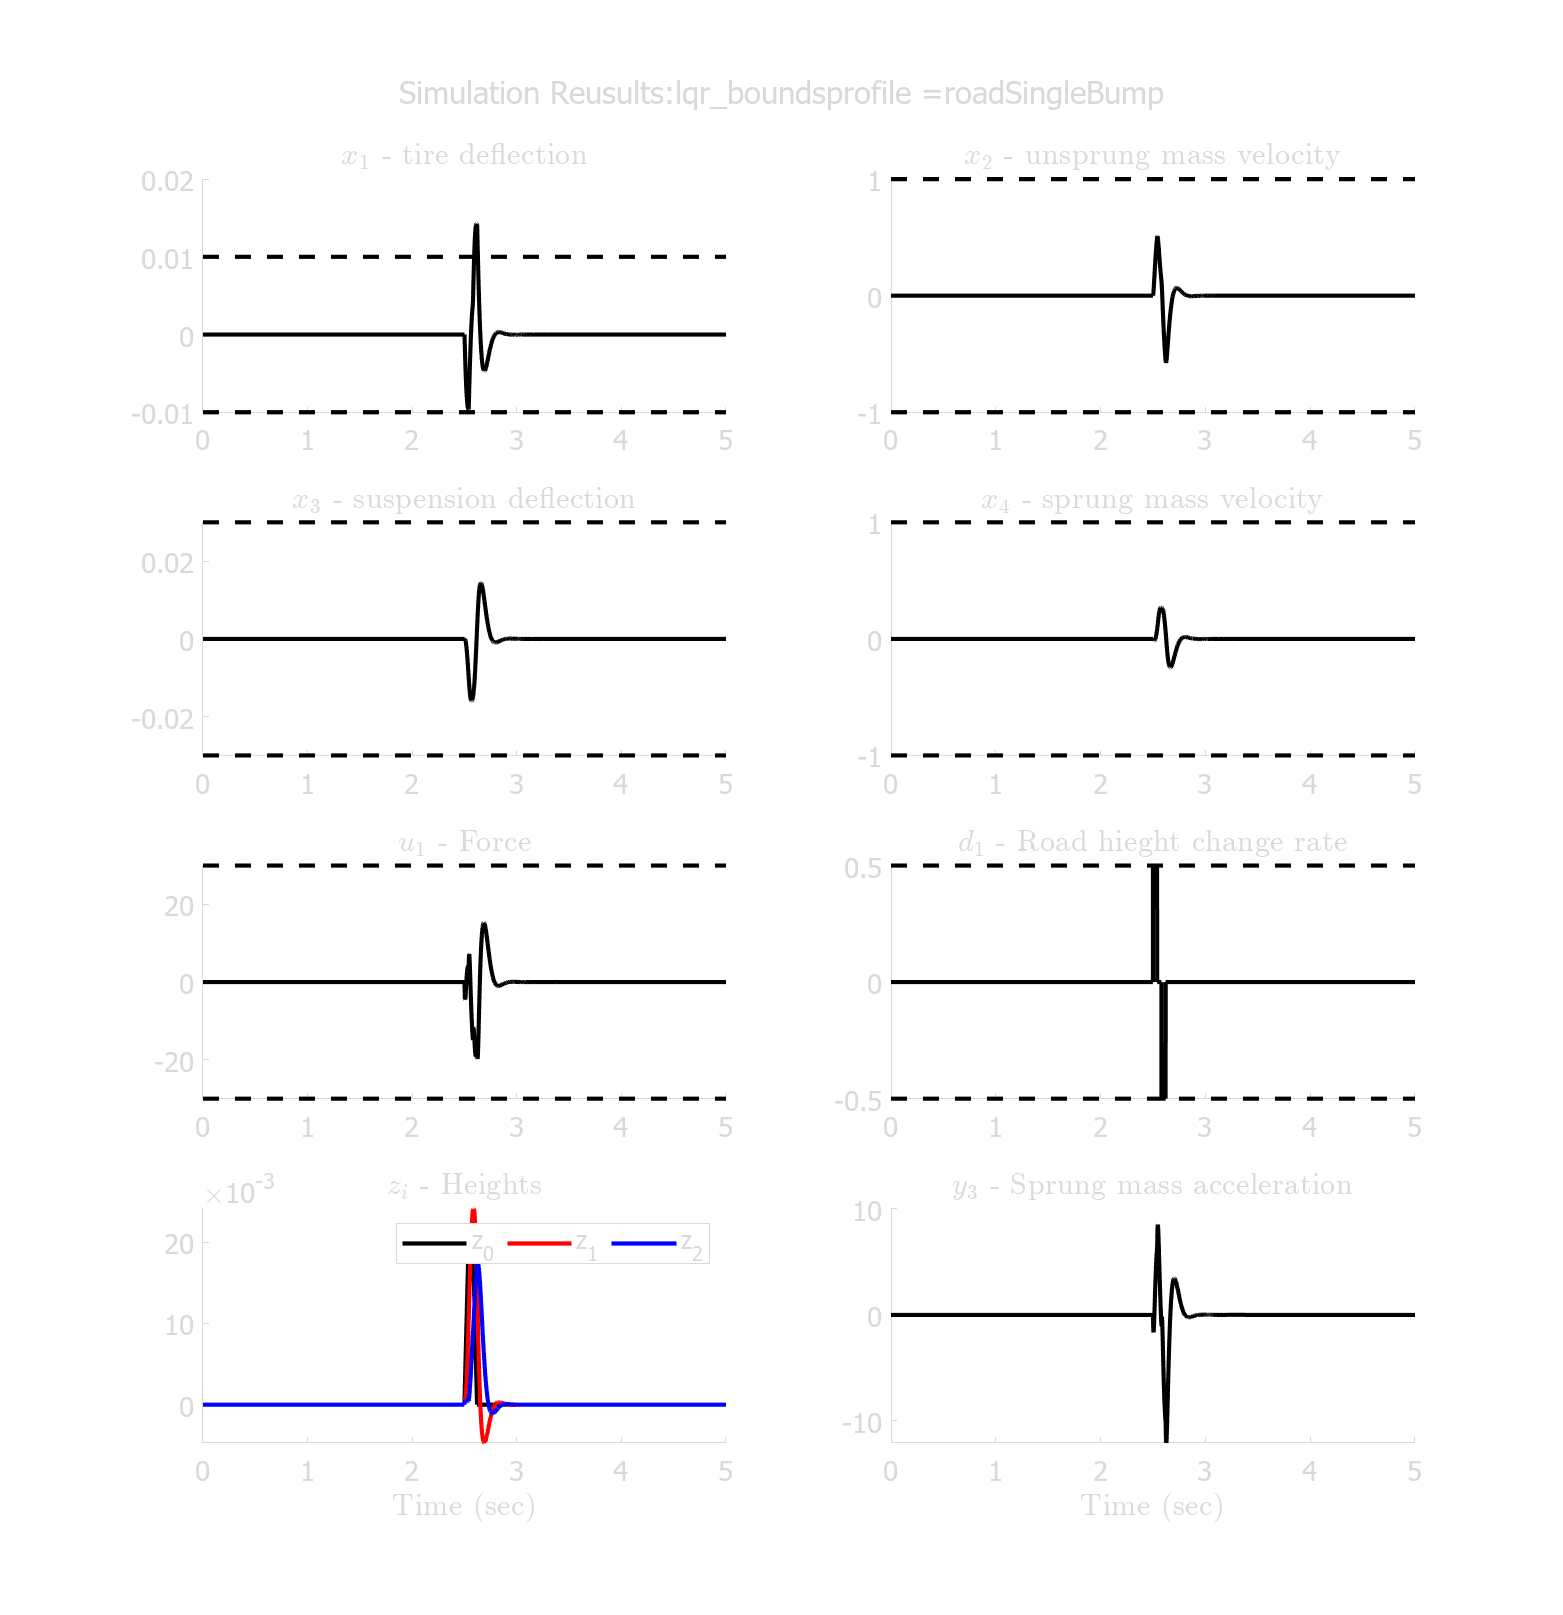
\includegraphics[width = 0.49 \columnwidth]{figs/results_lqr_bounds_roadSingleBump.png}
    \caption{LQR closed-loop dynamics with $Q_bounds$ and $R$ for the IRI\_737b  and roadBumpHole road profiles.} \label{fig:lqr_bounds}
\end{figure}

\begin{figure}[h]
    \centering
    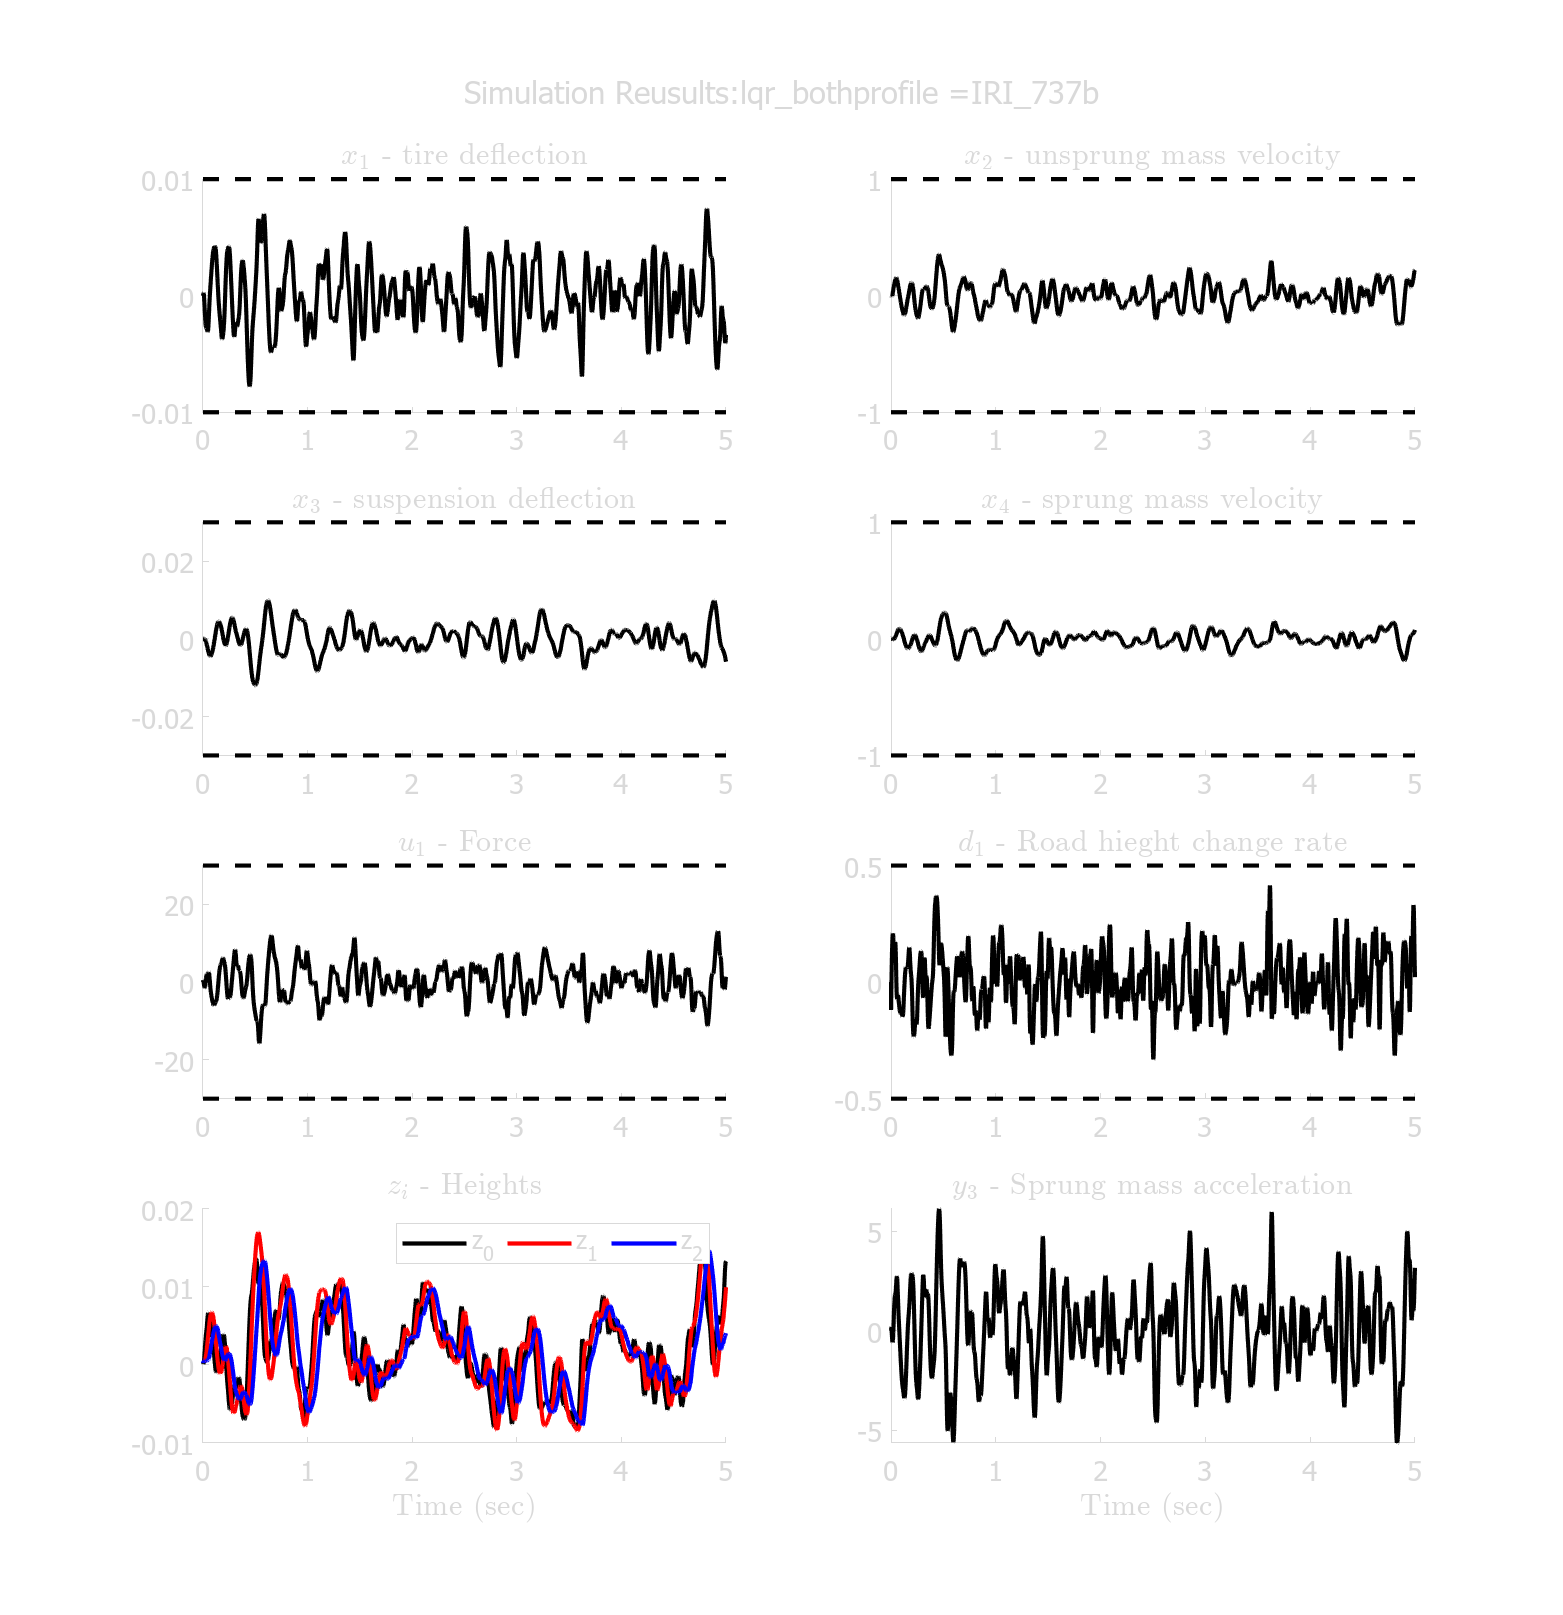
\includegraphics[width = 0.49 \columnwidth]{figs/results_lqr_both_IRI_737b.png}
    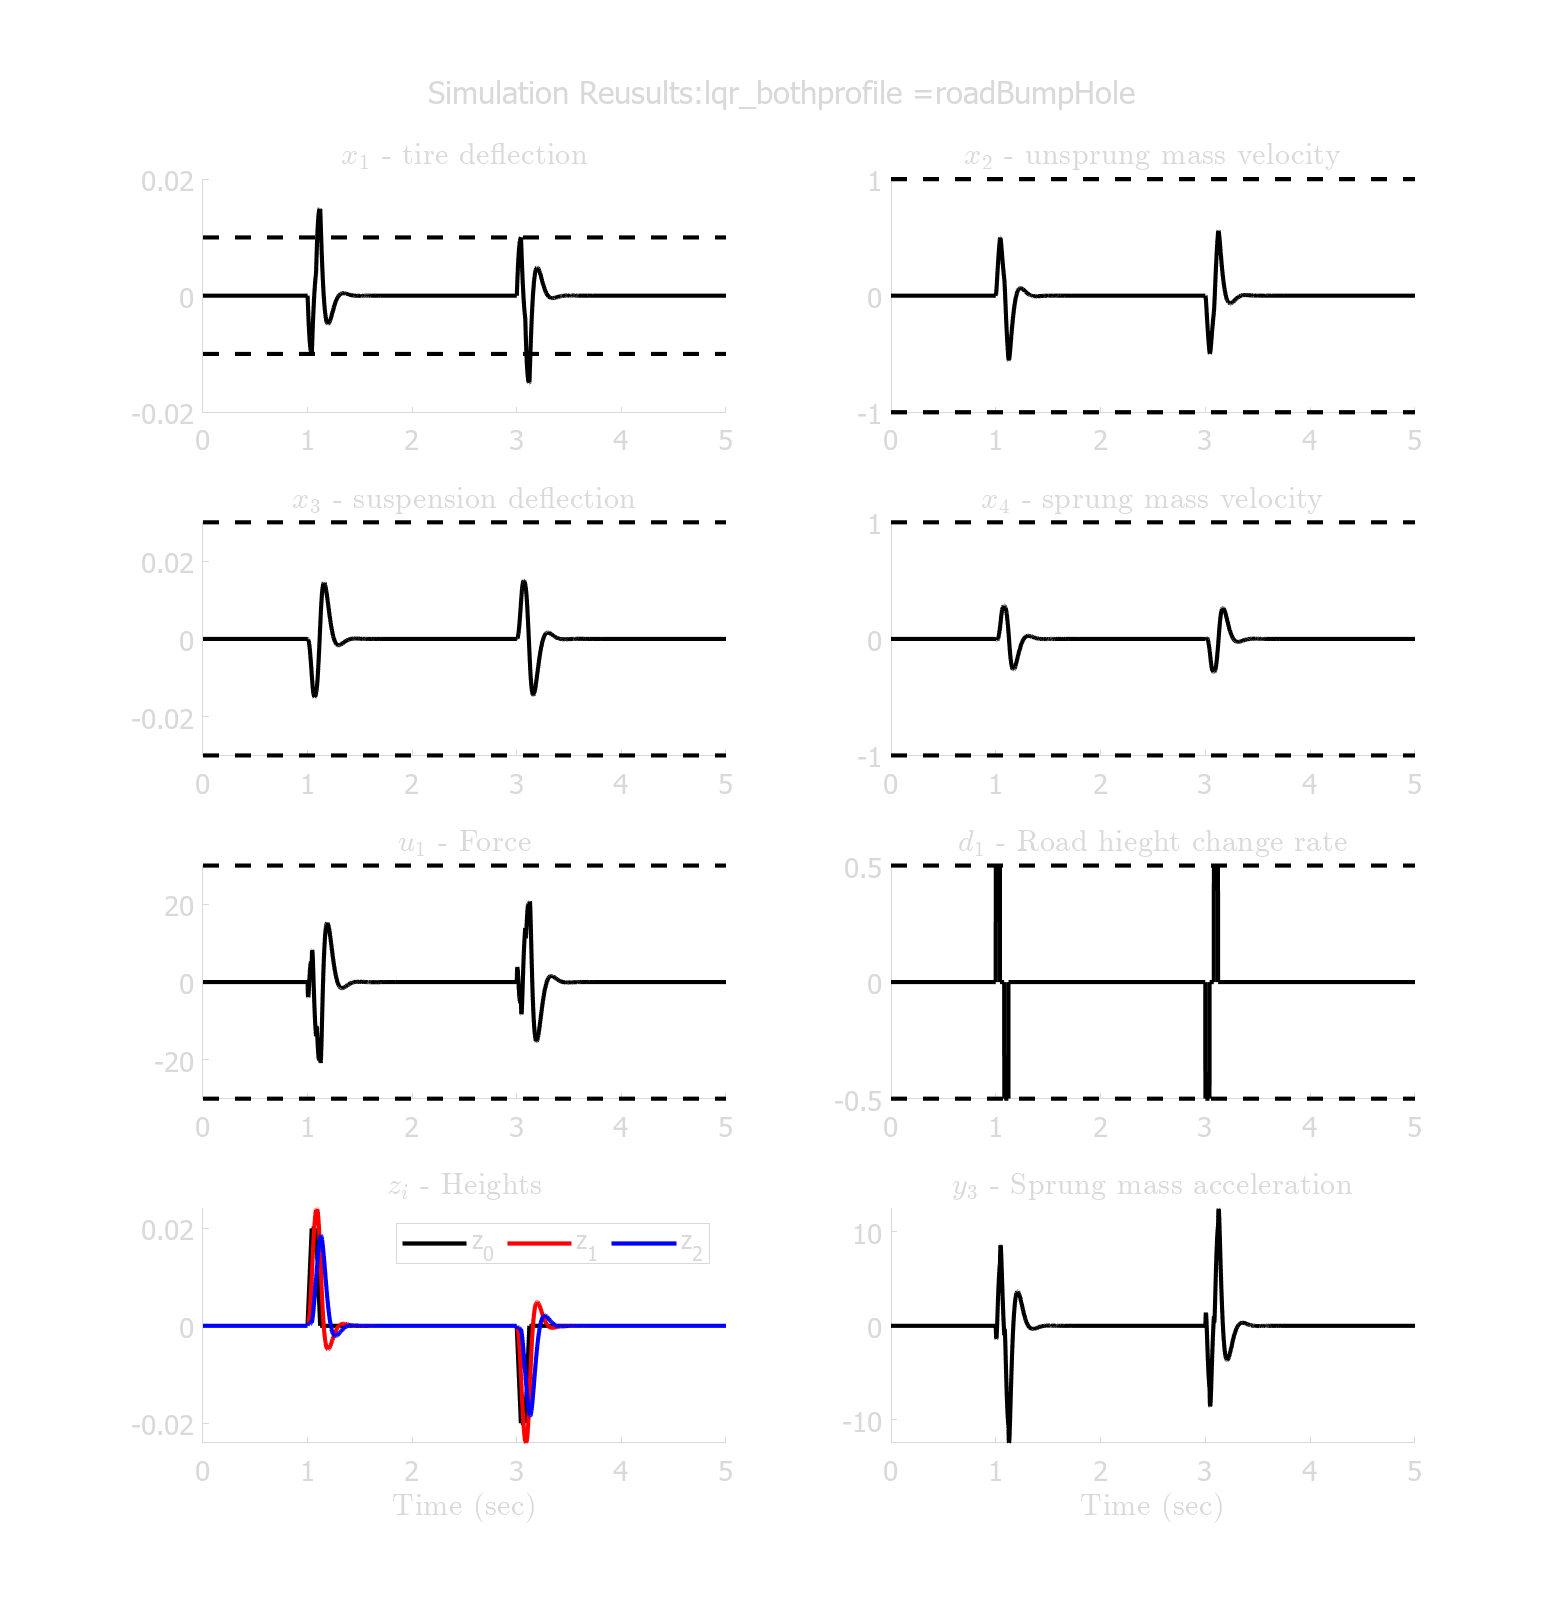
\includegraphics[width = 0.49 \columnwidth]{figs/results_lqr_both_roadBumpHole.png}
    % 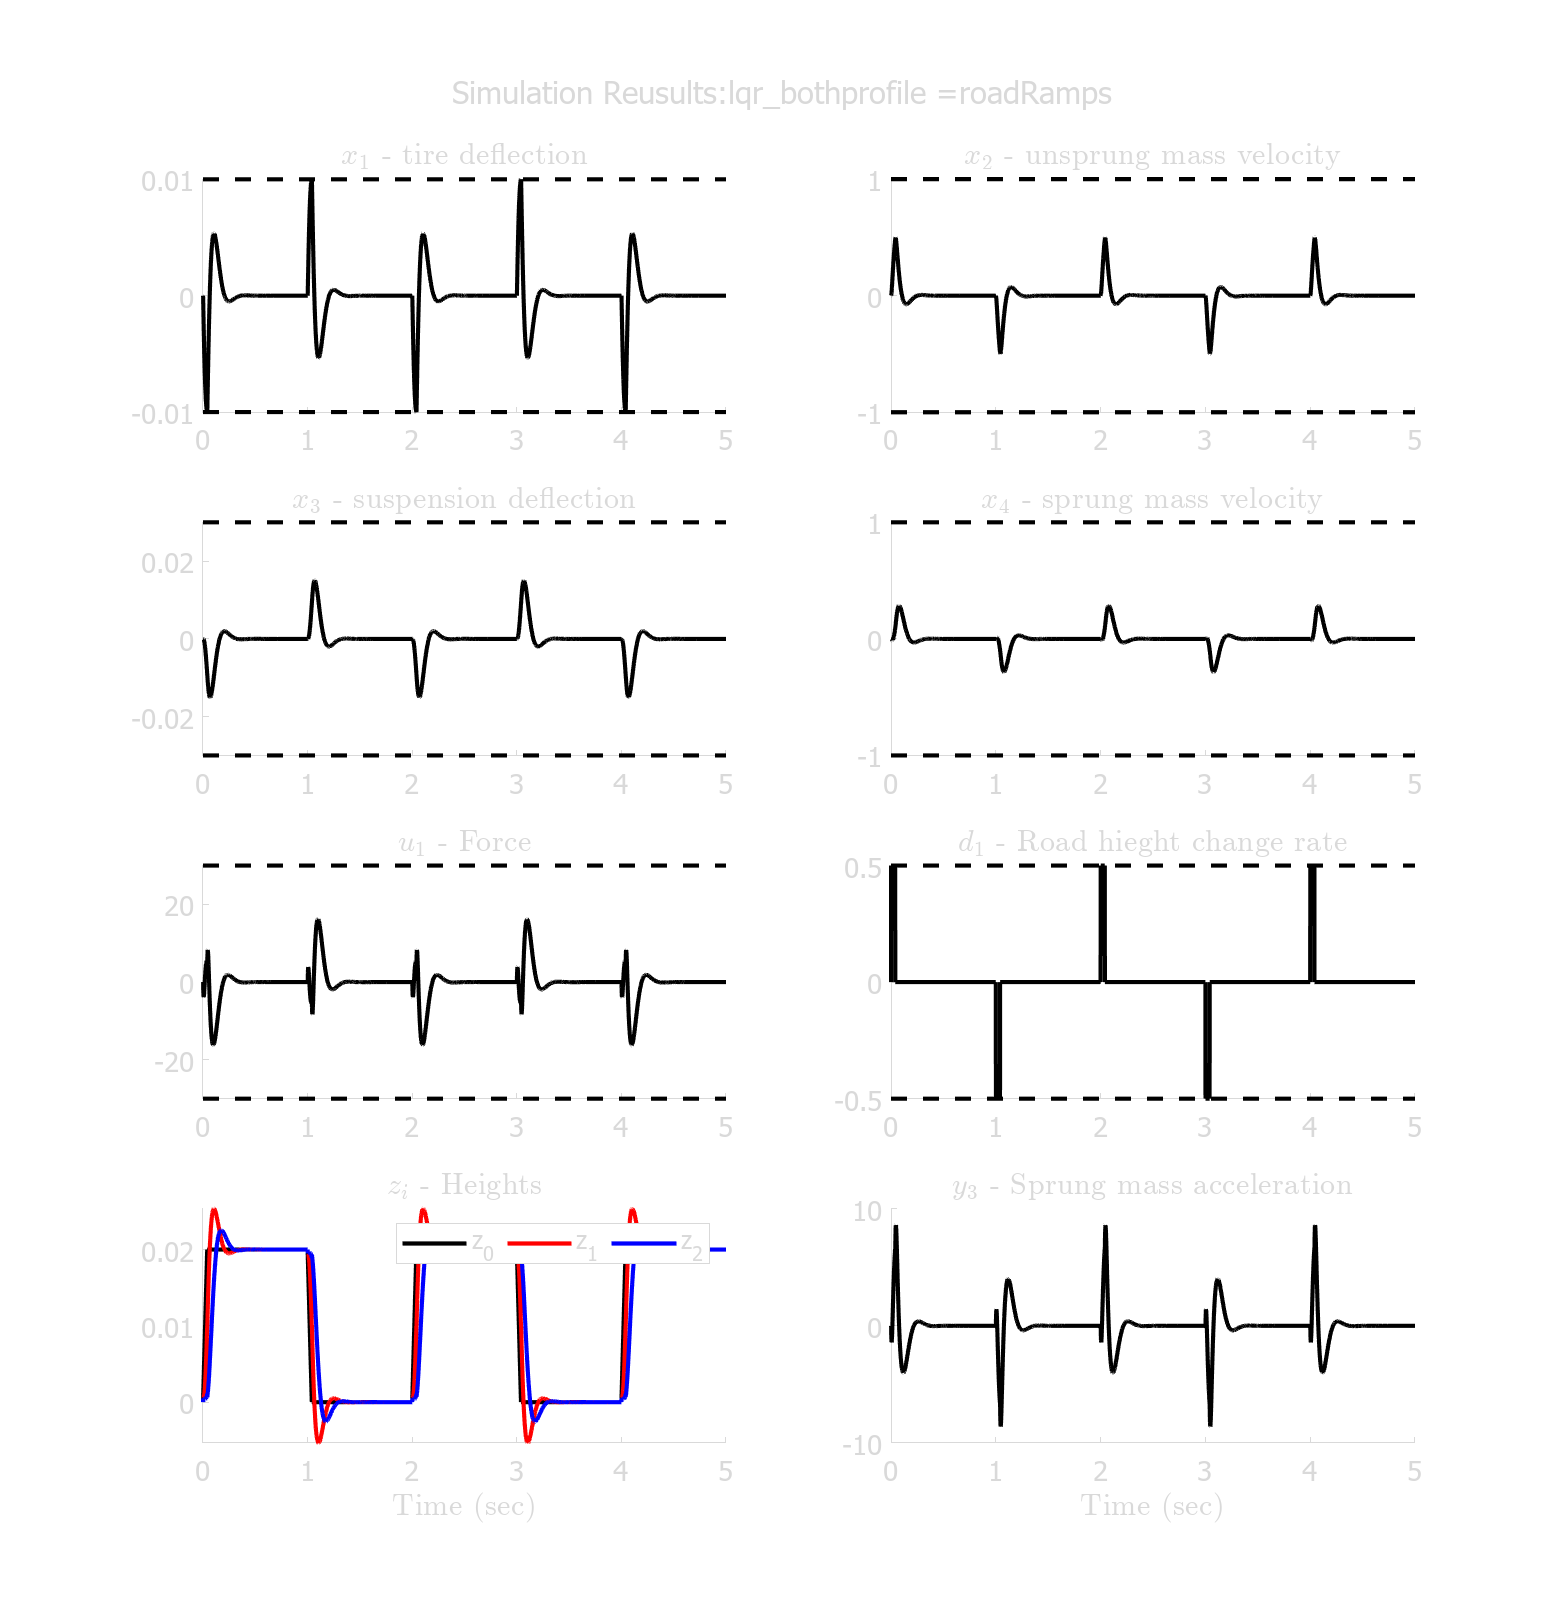
\includegraphics[width = 0.49 \columnwidth]{figs/results_lqr_both_roadRamps.png}
    % 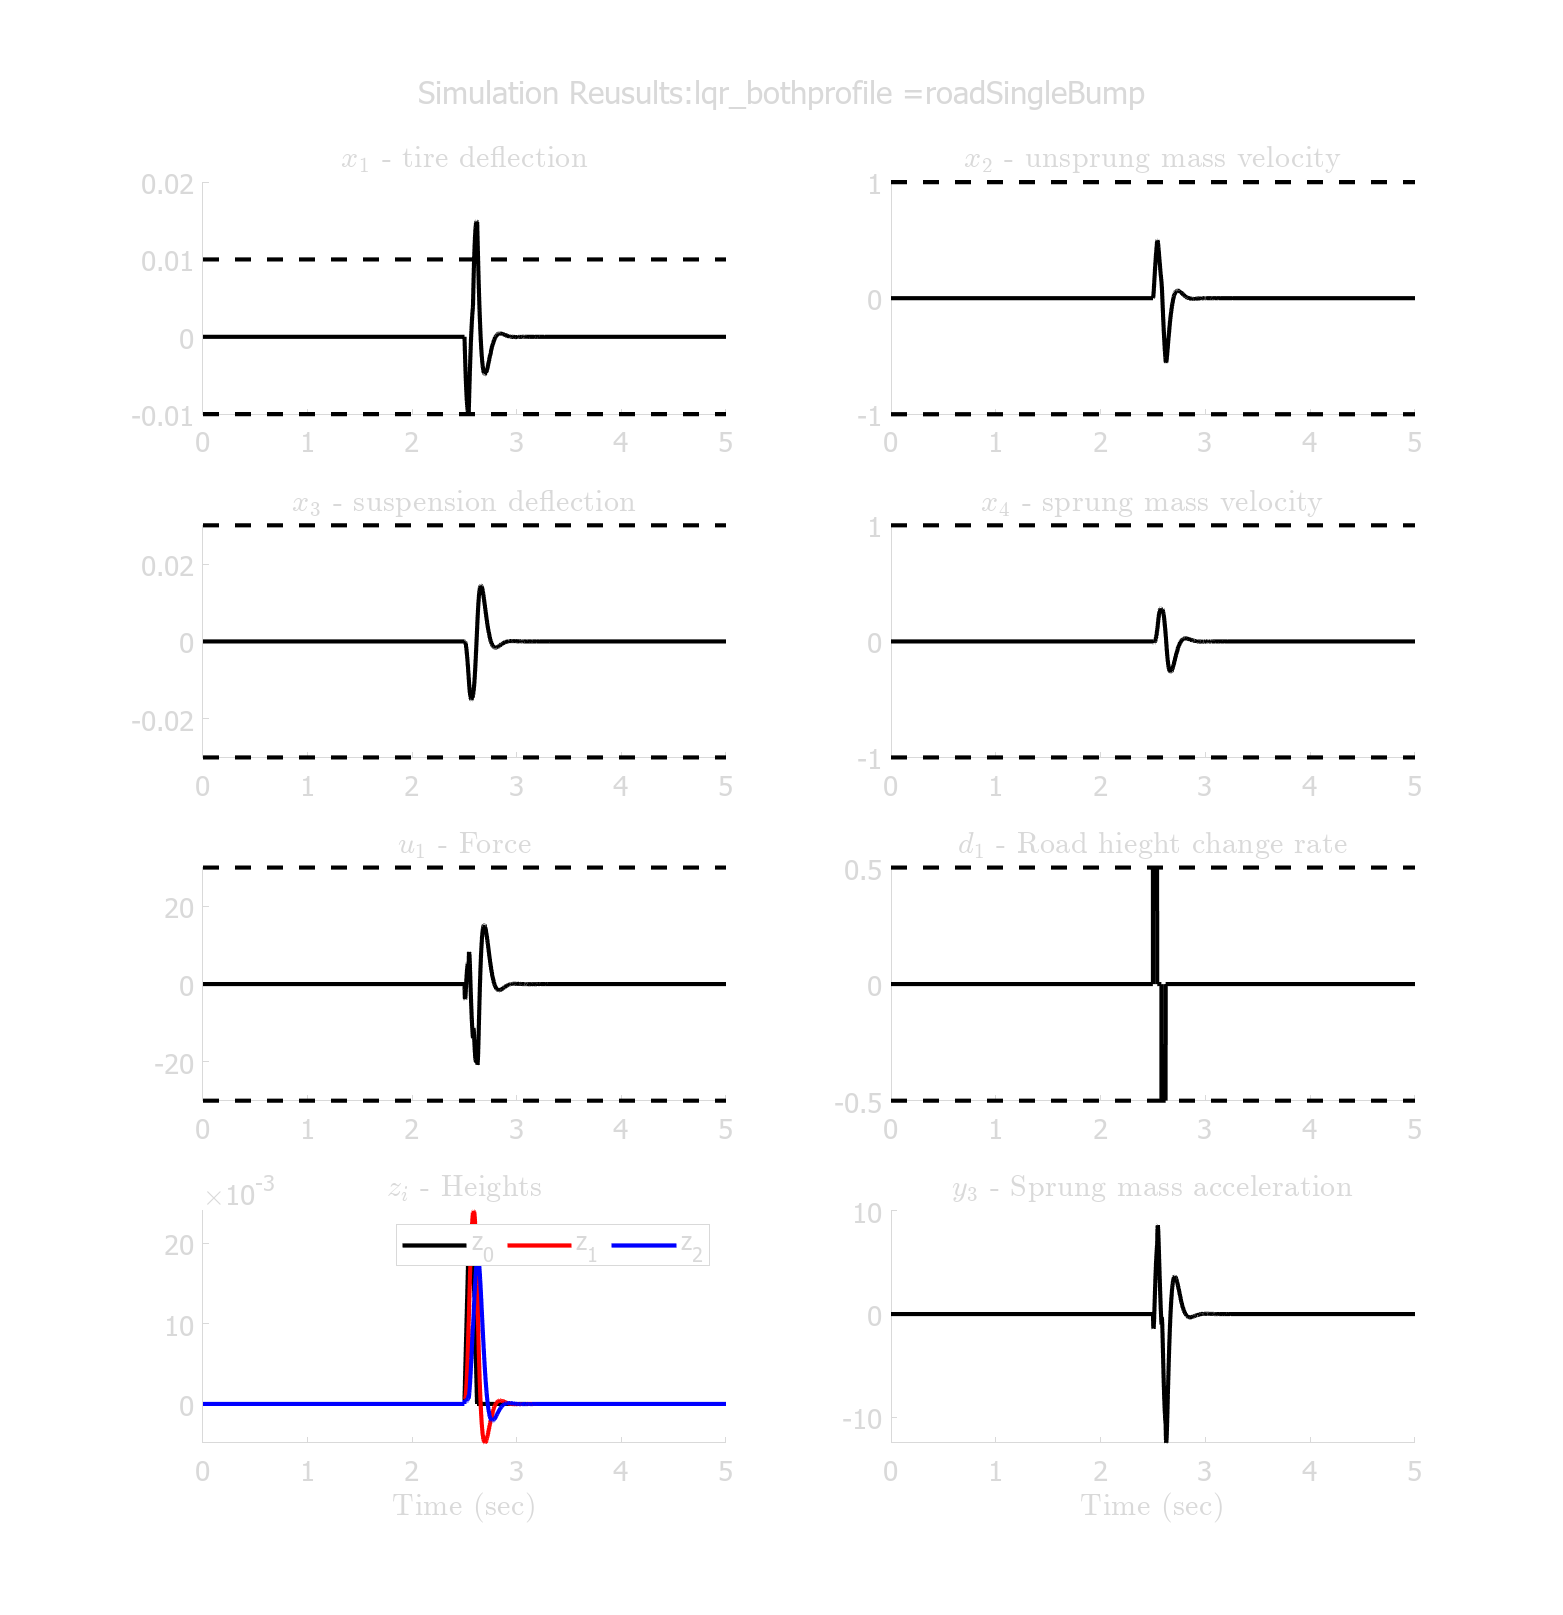
\includegraphics[width = 0.49 \columnwidth]{figs/results_lqr_both_roadSingleBump.png}
    \caption{LQR closed-loop dynamics with $Q_both$ and $R$ for the IRI\_737b  and roadBumpHole road profiles.} \label{fig:lqr_both}
\end{figure}

Each of these lqr control schemes had a noticeable improvement in dampening transient response.
The demonstrative $Q$ matrices are weighted against the $R$ matrices by multiple orders of magnitude as iteratively testing yielded these weights to have a reasonable balance.

Although it does have a noticeable improvement in response, it does not meet the ideal specs; specifically, the state bounds are still often exceeded and the oscillations still don't seem like an enjoyable ride.

\newpage
% -----------------------------------------------------
% Simple MPC Controller Formulation
% -----------------------------------------------------
\section{Simple MPC Controller Formulation}
An initial implementation of the MPC controller was constructed using the provided code.
The same $Q$ and $R$ matrices from before were used and tested iteratively to attempt good responses.
(See MATLAB code with rFlag = 0 for the simple formulation).
For demonstrative purposes only the $Q_{both}$ version of cost are provided in this report.

\subsection{Update Parameter Selection}
The time-horizon and time-step selection were tested for multiple values and ultimately the decision to select a specific value for this was pretty arbitrary.
The demonstrative plots are using $N=15$, but this selection was mostly just an initial guess and since no explicit hardware was selected the computational limit is pretty arbitrary.
The integer multiplier was selected mainly by comparing a few different values.
As can be seen in \autoref{fig:mpc_N15_dt1_d0_r0}, the case where the prediction forward is done every-single time-step the response becomes very oscillatory and the bounds are greatly exceeded.

\begin{figure}[h]
    \centering
    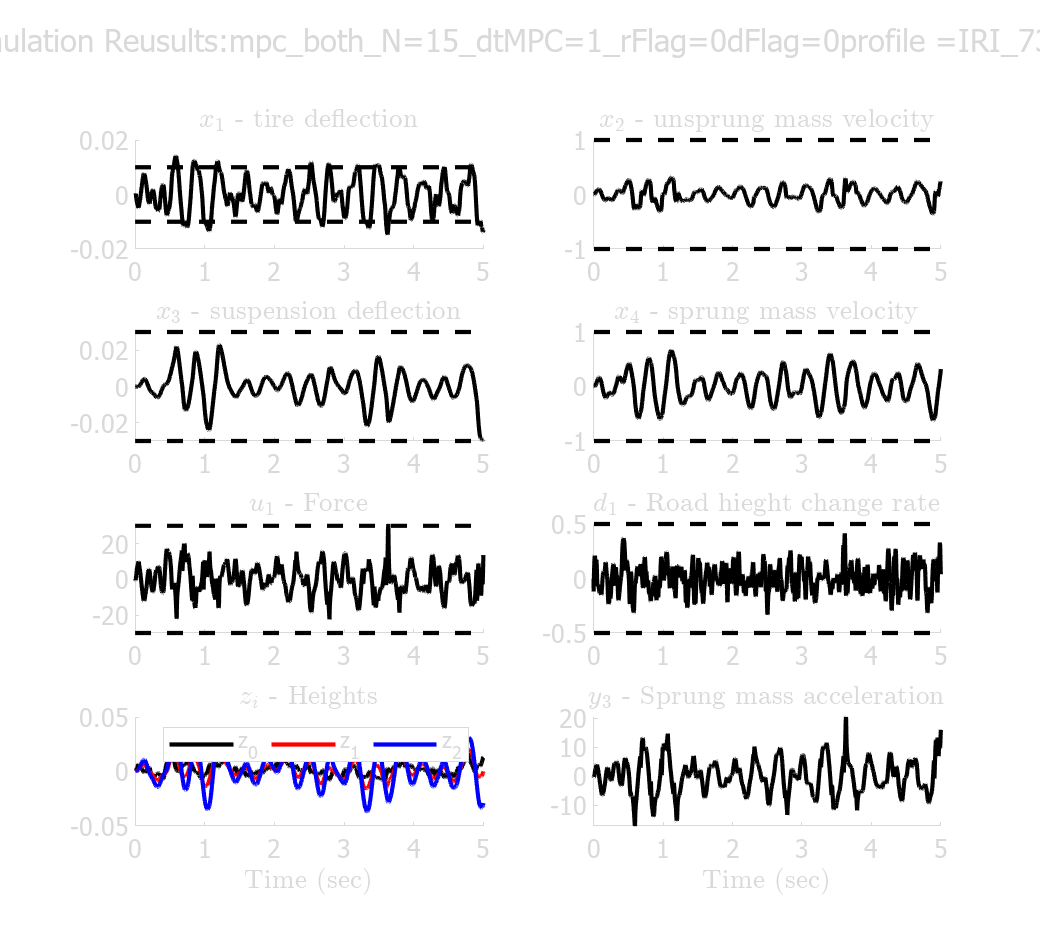
\includegraphics[width = 0.49 \columnwidth]{figs/results_mpc_both_N=15_dtMPC=1_rFlag=0_dFlag=0_IRI_737b.png}
    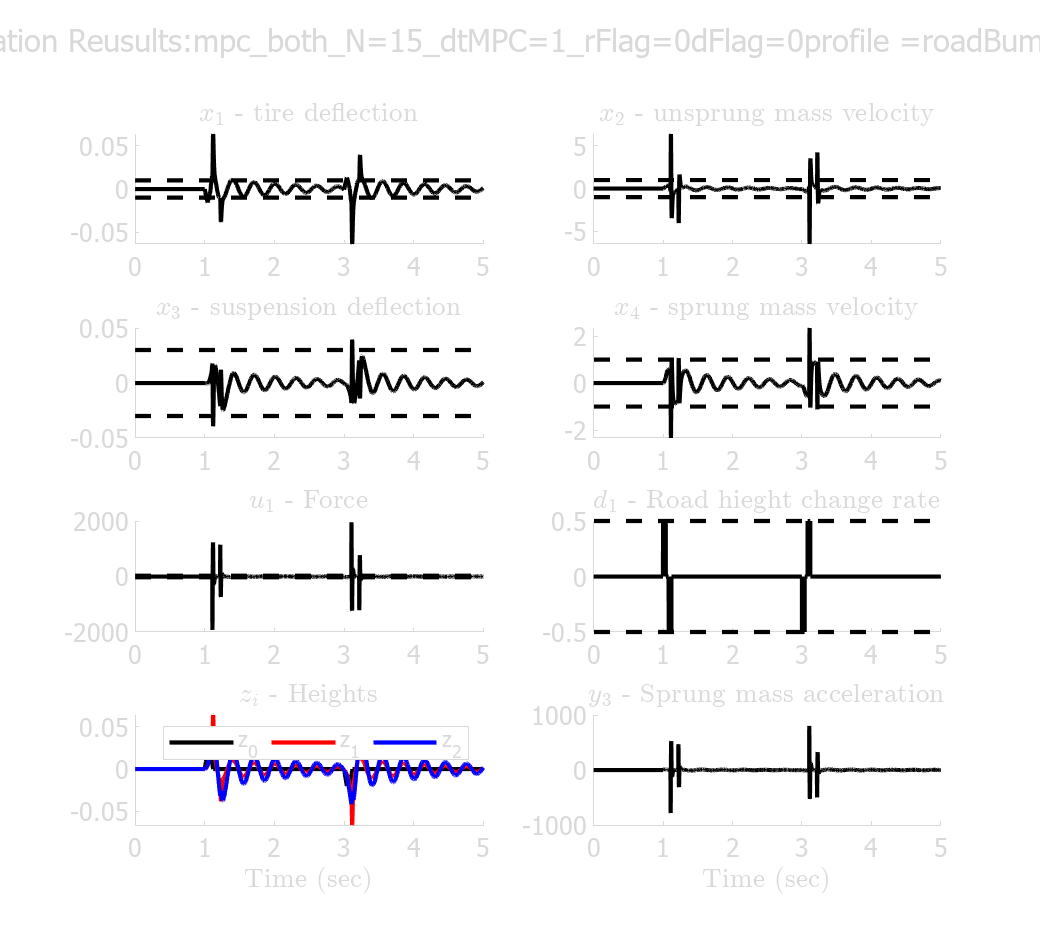
\includegraphics[width = 0.49 \columnwidth]{figs/results_mpc_both_N=15_dtMPC=1_rFlag=0_dFlag=0_roadBumpHole.png}
    % 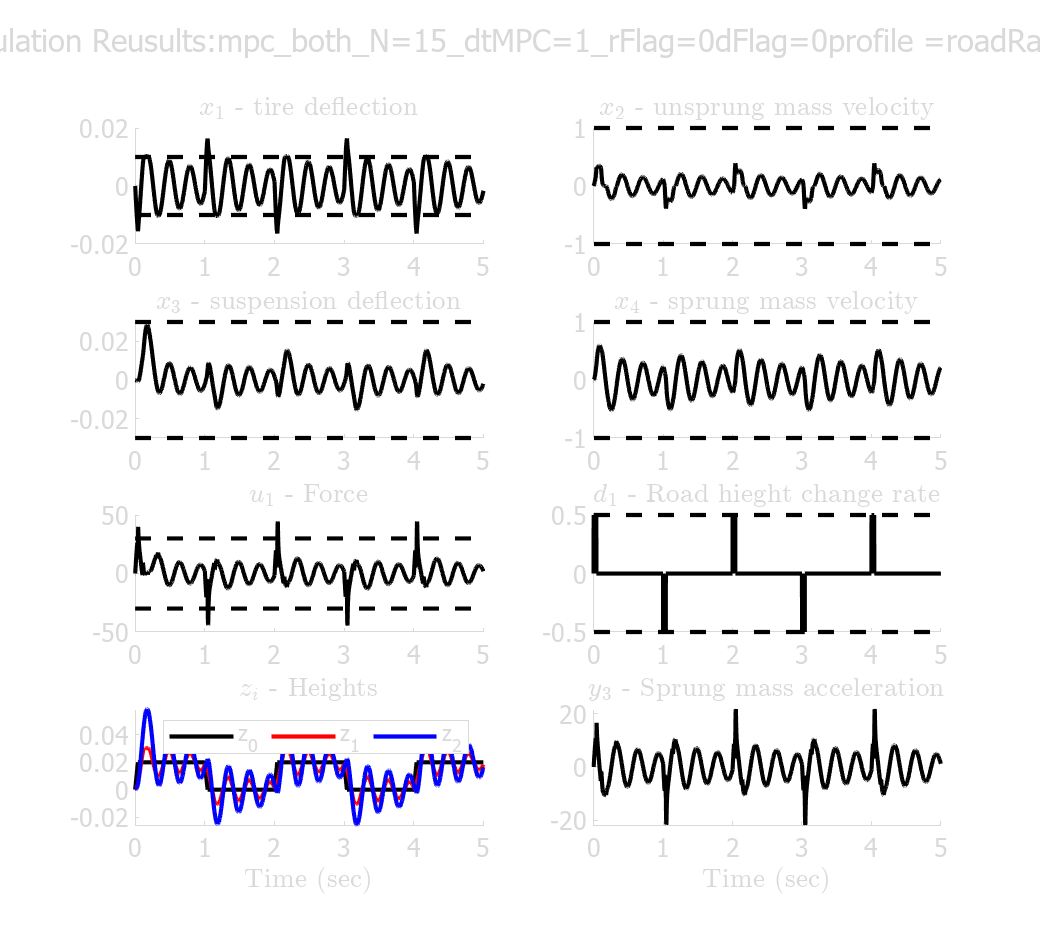
\includegraphics[width = 0.49 \columnwidth]{figs/results_mpc_both_N=15_dtMPC=1_rFlag=0_dFlag=0_roadRamps.png}
    % 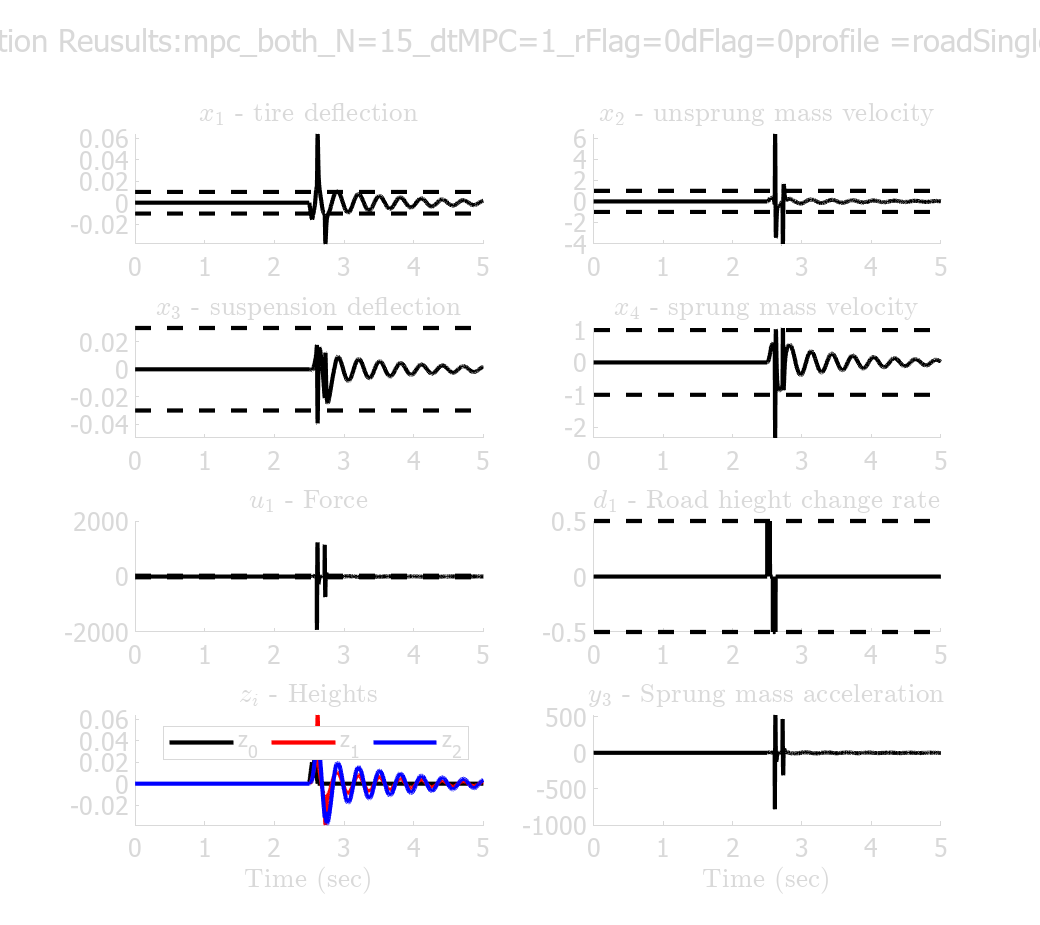
\includegraphics[width = 0.49 \columnwidth]{figs/results_mpc_both_N=15_dtMPC=1_rFlag=0_dFlag=0_roadSingleBump.png}
    \caption{Closed-loop dynamics with no disturbance information for standard MPC using $Q_both$ and $R$ updating every time-step with $N=15$ for the IRI\_737b and roadBumpHole road profiles.} \label{fig:mpc_N15_dt1_d0_r0}
\end{figure}

By comparison, as seen in \autoref{fig:mpc_N15_dt3_d0_r0}, predicting forward in increments of 3 time-steps is far less oscillatory; however this is also dependent on what $N$ is.

\begin{figure}[h]
    \centering
    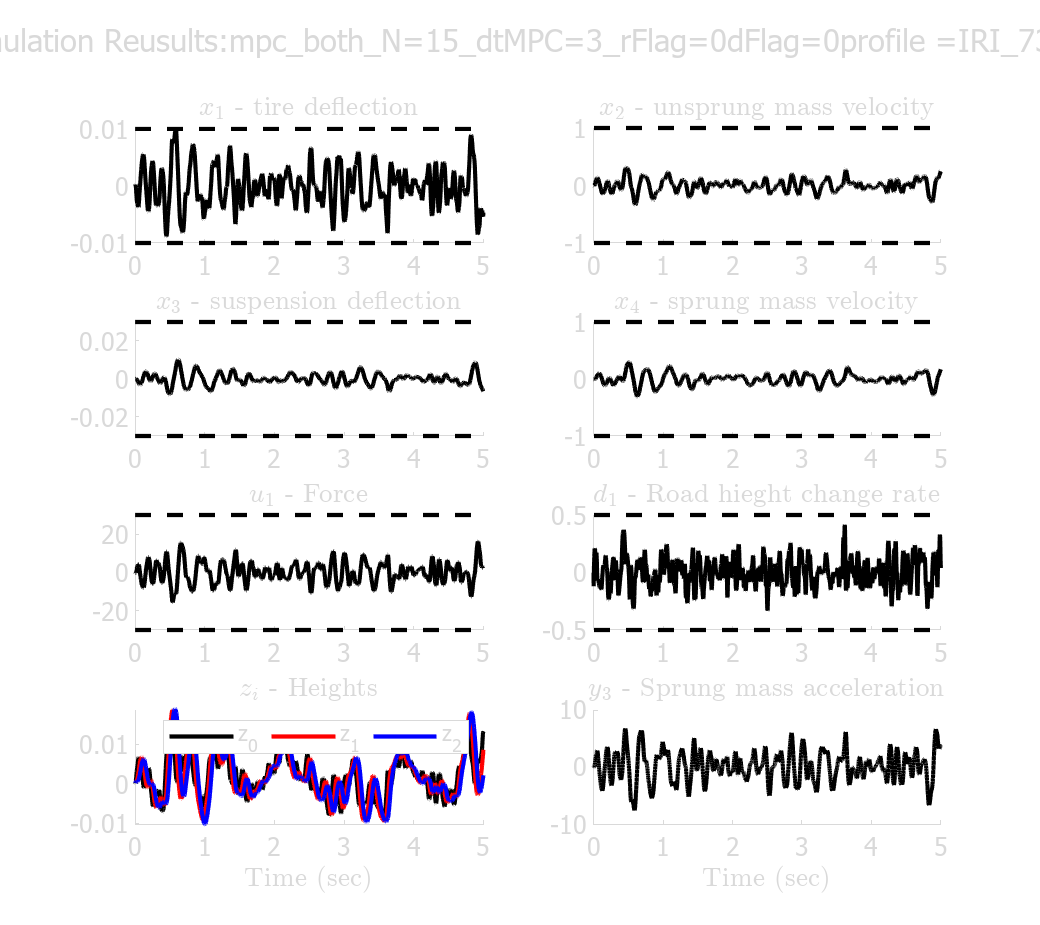
\includegraphics[width = 0.49 \columnwidth]{figs/results_mpc_both_N=15_dtMPC=3_rFlag=0_dFlag=0_IRI_737b.png}
    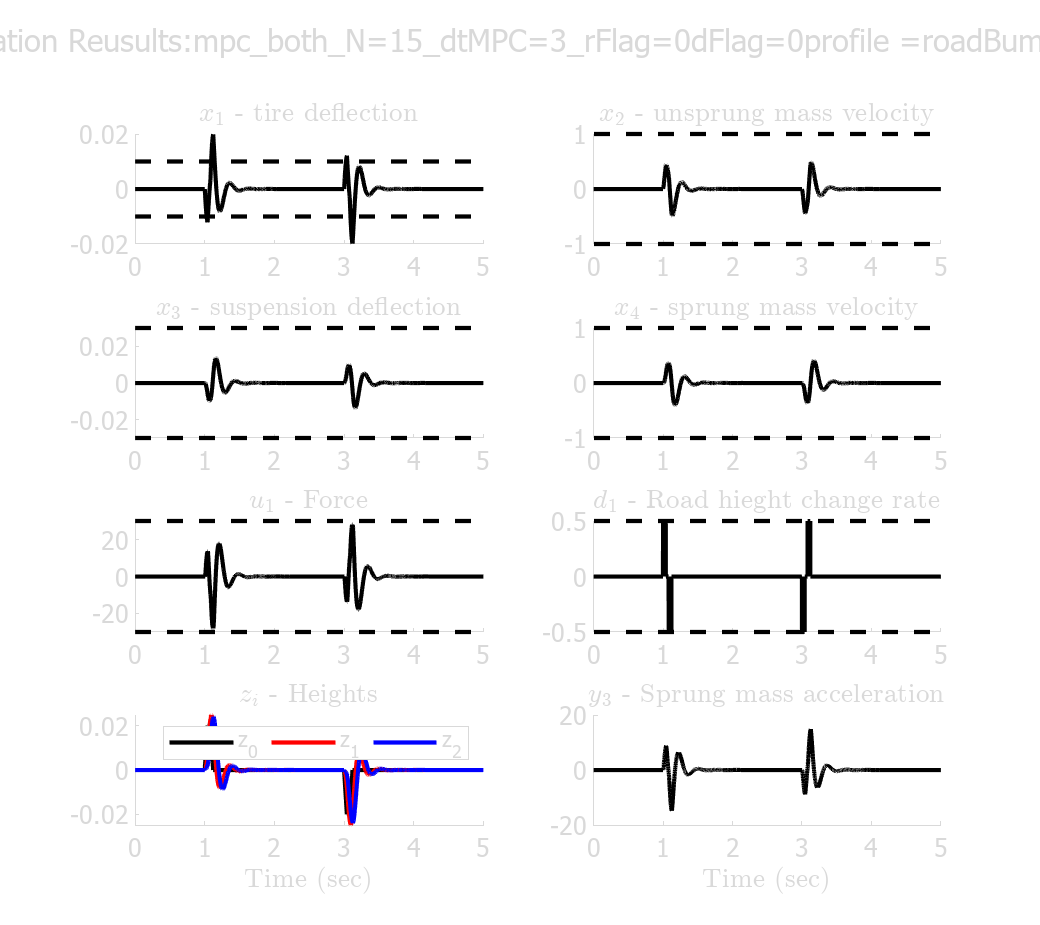
\includegraphics[width = 0.49 \columnwidth]{figs/results_mpc_both_N=15_dtMPC=3_rFlag=0_dFlag=0_roadBumpHole.png}
    % 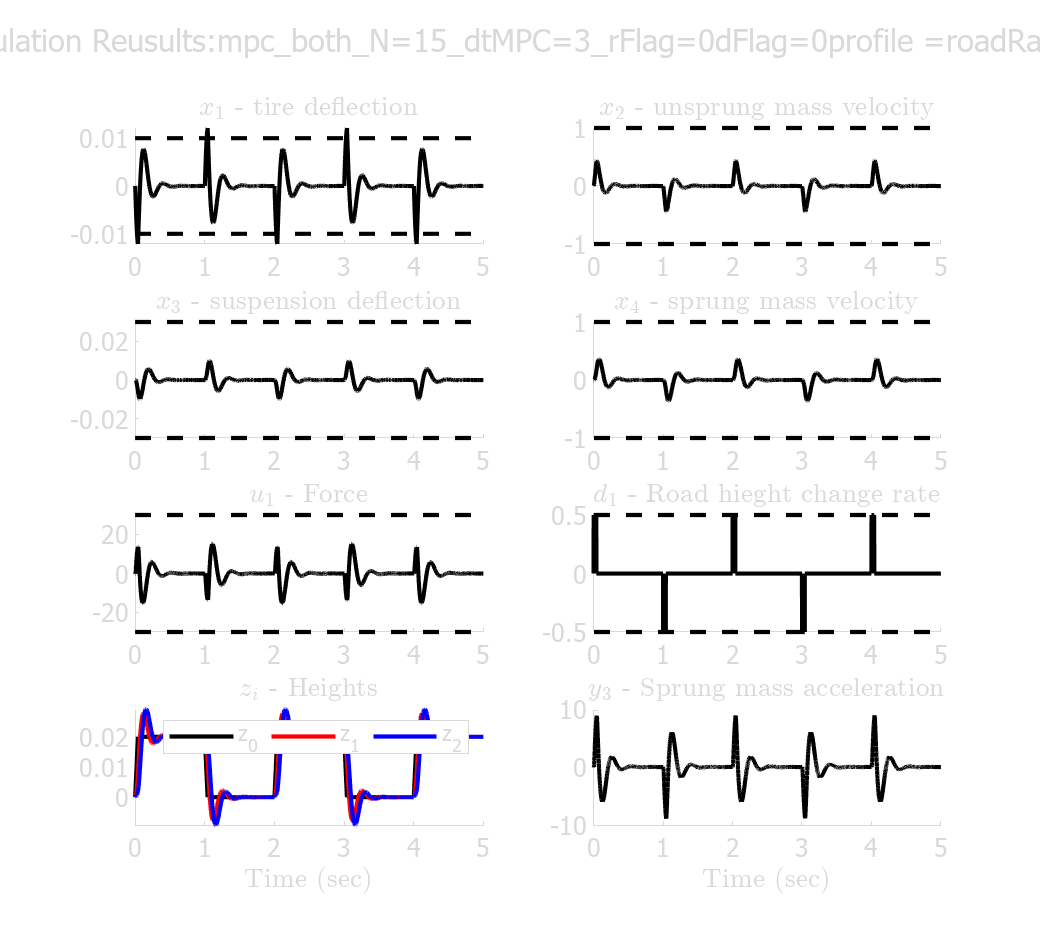
\includegraphics[width = 0.49 \columnwidth]{figs/results_mpc_both_N=15_dtMPC=3_rFlag=0_dFlag=0_roadRamps.png}
    % 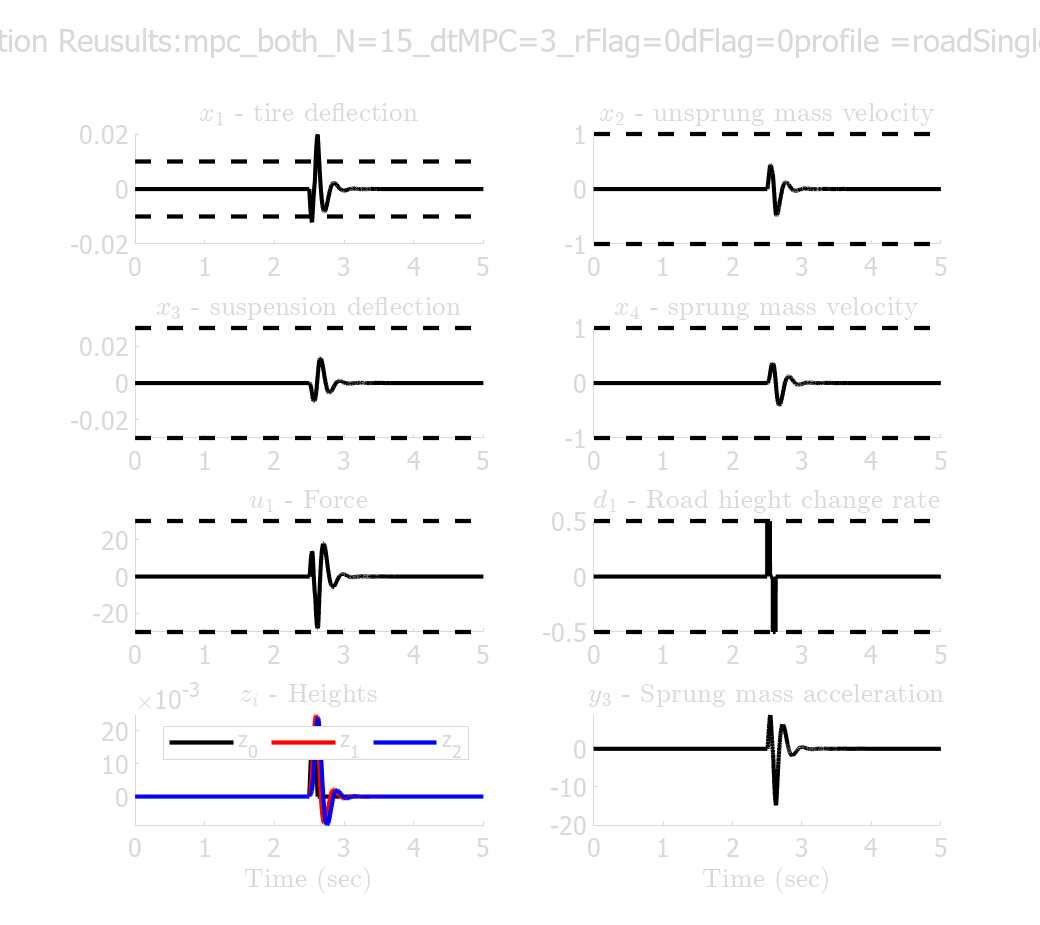
\includegraphics[width = 0.49 \columnwidth]{figs/results_mpc_both_N=15_dtMPC=3_rFlag=0_dFlag=0_roadSingleBump.png}
    \caption{Closed-loop dynamics with no disturbance information for standard MPC using $Q_both$ and $R$ updating every 3 time-steps with $N=15$ for the IRI\_737b and roadBumpHole road profiles.} \label{fig:mpc_N15_dt3_d0_r0}
\end{figure}

\subsection{Disturbance knowledge Comparison}
The closed-loop dynamics were also tested for when the MPC is given different levels of disturbance information:
\begin{enumerate}
    \item The nominal case (dFlag = 0) sets $d_1 = d_2 = 0$ for the entire time-horizon.
    \item The current state-known case (dFlag = 1) assumes that $d_1$ and $d_2$ are known at $k$. Although also tested when the rest of the testing-horizon is fully nominal ($d_1 = d_2 = 0$) and $d_1 = 0$ for the rest of the horizon, the better approach was for $d_2$ to be derived from having $d_1$ held constant for the time-horizon.
    \item The entire knowledge case (dFlag = 2) has both $d_1$ and $d_2$ directly inputed into the MPC problem.
\end{enumerate}

A direct comparison can be seen in \autoref{fig:mpc_N15_dt3_d1_r0},\autoref{fig:mpc_N15_dt3_d1_r0}, and \autoref{fig:mpc_N15_dt3_d2_r0}. 

\begin{figure}[h]
    \centering
    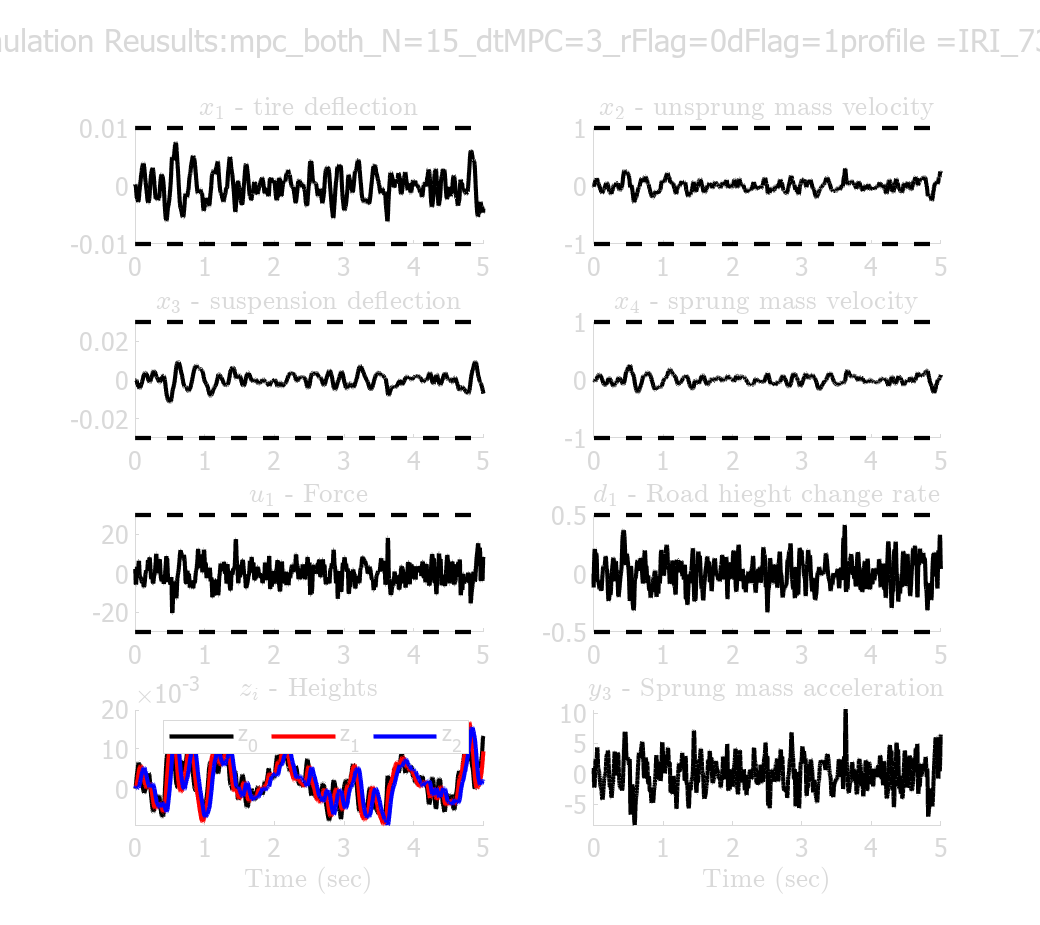
\includegraphics[width = 0.49 \columnwidth]{figs/results_mpc_both_N=15_dtMPC=3_rFlag=0_dFlag=1_IRI_737b.png}
    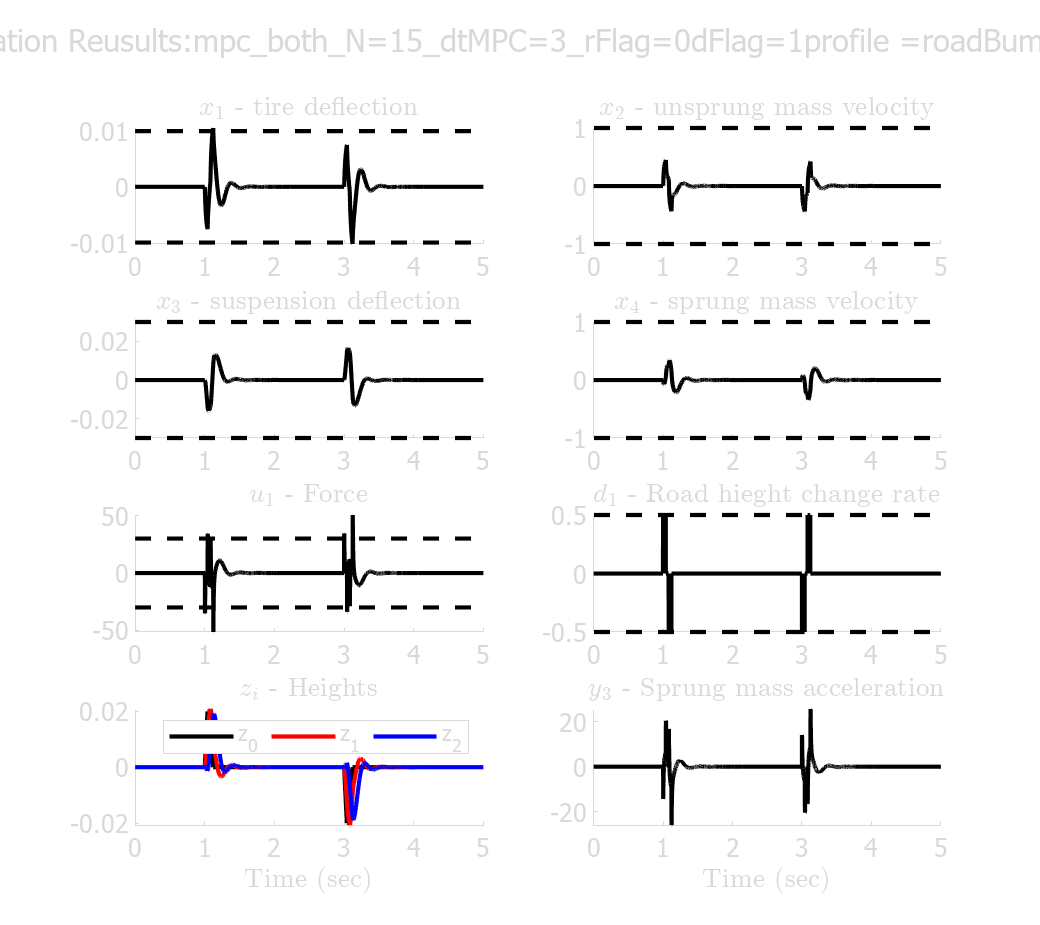
\includegraphics[width = 0.49 \columnwidth]{figs/results_mpc_both_N=15_dtMPC=3_rFlag=0_dFlag=1_roadBumpHole.png}
    % 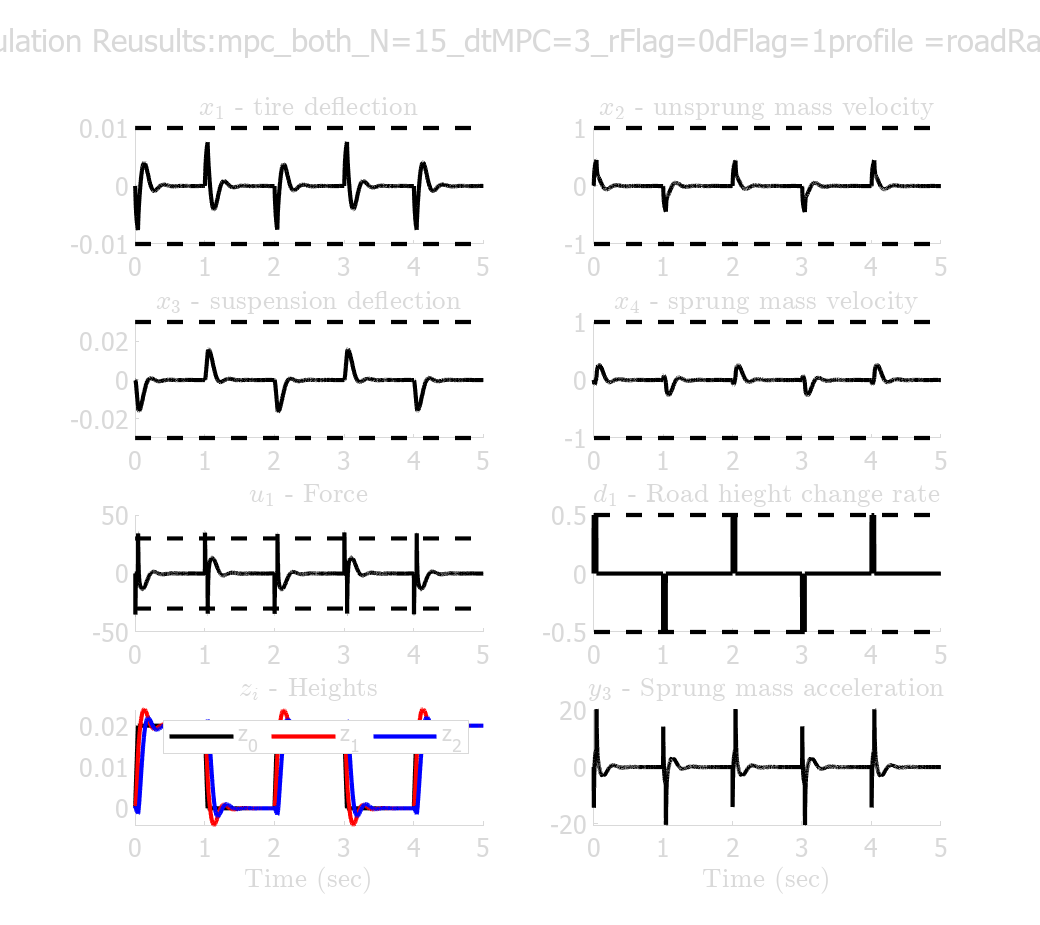
\includegraphics[width = 0.49 \columnwidth]{figs/results_mpc_both_N=15_dtMPC=3_rFlag=0_dFlag=1_roadRamps.png}
    % 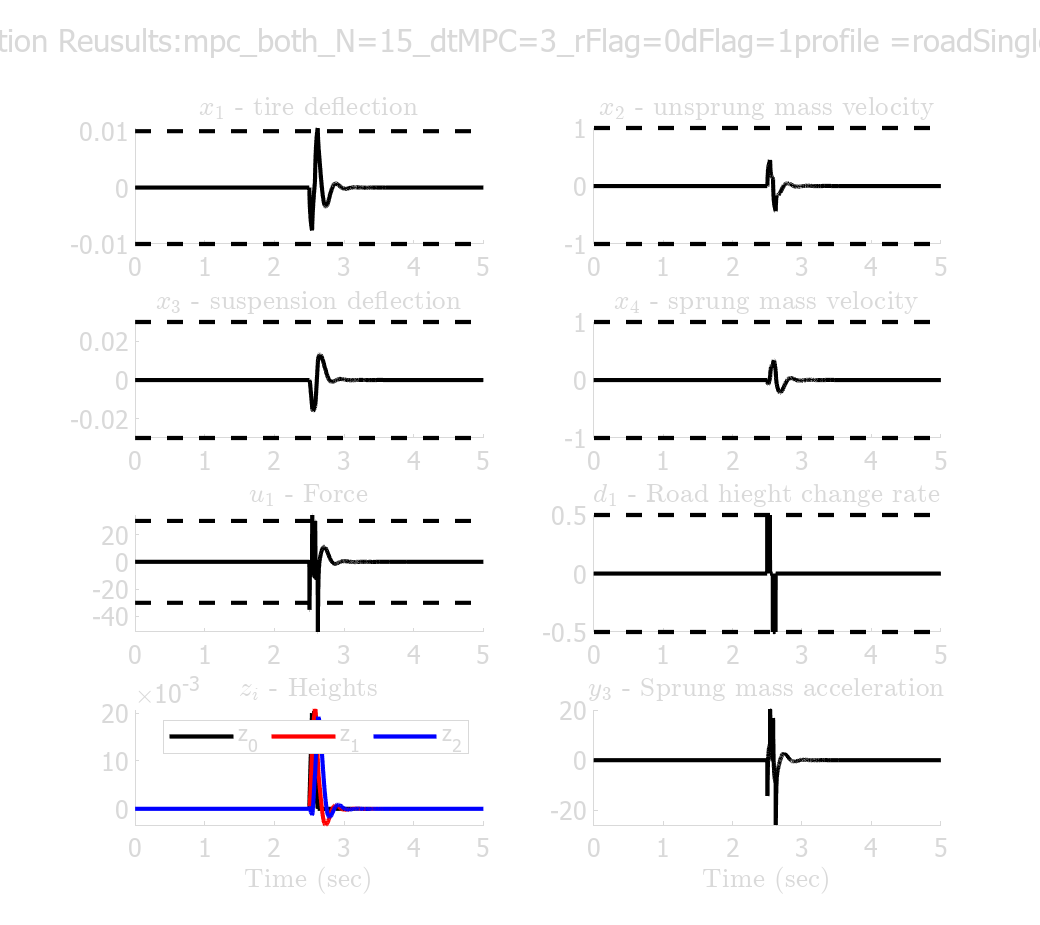
\includegraphics[width = 0.49 \columnwidth]{figs/results_mpc_both_N=15_dtMPC=3_rFlag=0_dFlag=1_roadSingleBump.png}
    \caption{Closed-loop dynamics with partial disturbance information for standard MPC using $Q_both$ and $R$ updating every 3 time-steps with $N=15$ for the IRI\_737b and roadBumpHole road profiles.} \label{fig:mpc_N15_dt3_d1_r0}
\end{figure}

\begin{figure}[h]
    \centering
    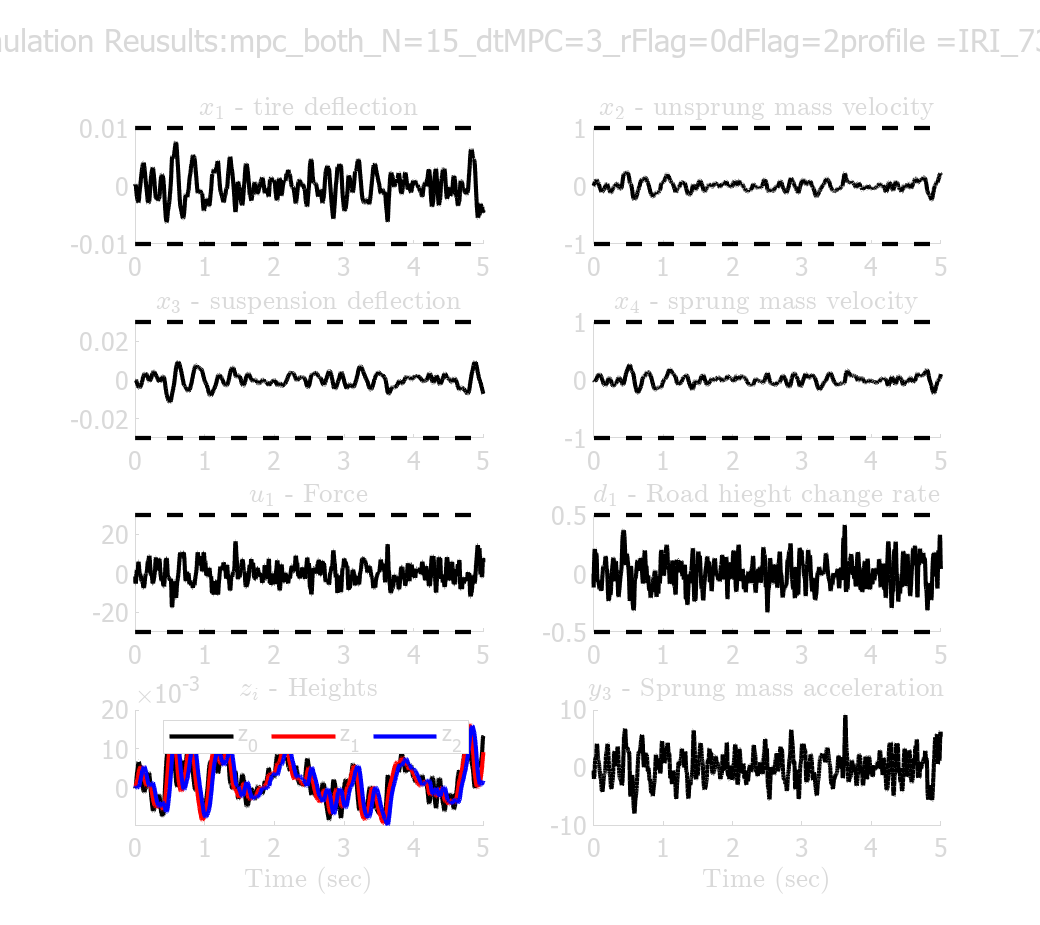
\includegraphics[width = 0.49 \columnwidth]{figs/results_mpc_both_N=15_dtMPC=3_rFlag=0_dFlag=2_IRI_737b.png}
    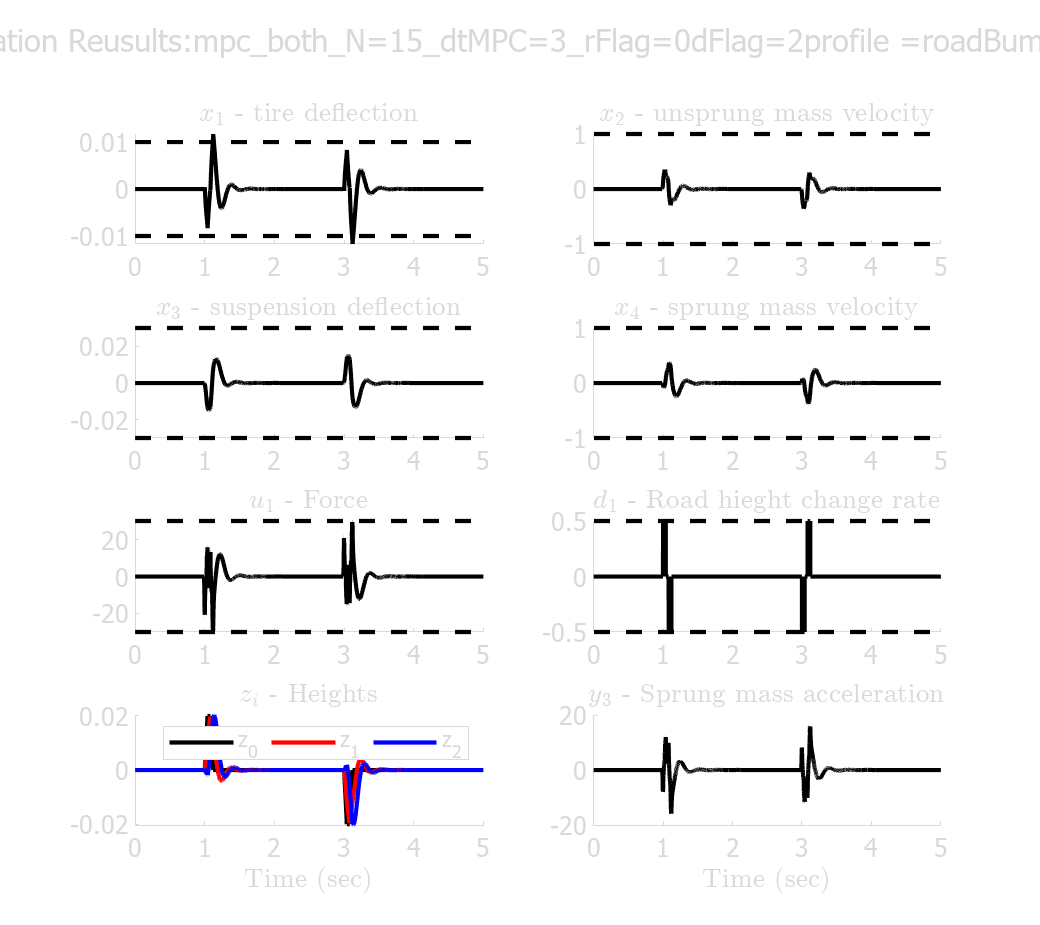
\includegraphics[width = 0.49 \columnwidth]{figs/results_mpc_both_N=15_dtMPC=3_rFlag=0_dFlag=2_roadBumpHole.png}
    % 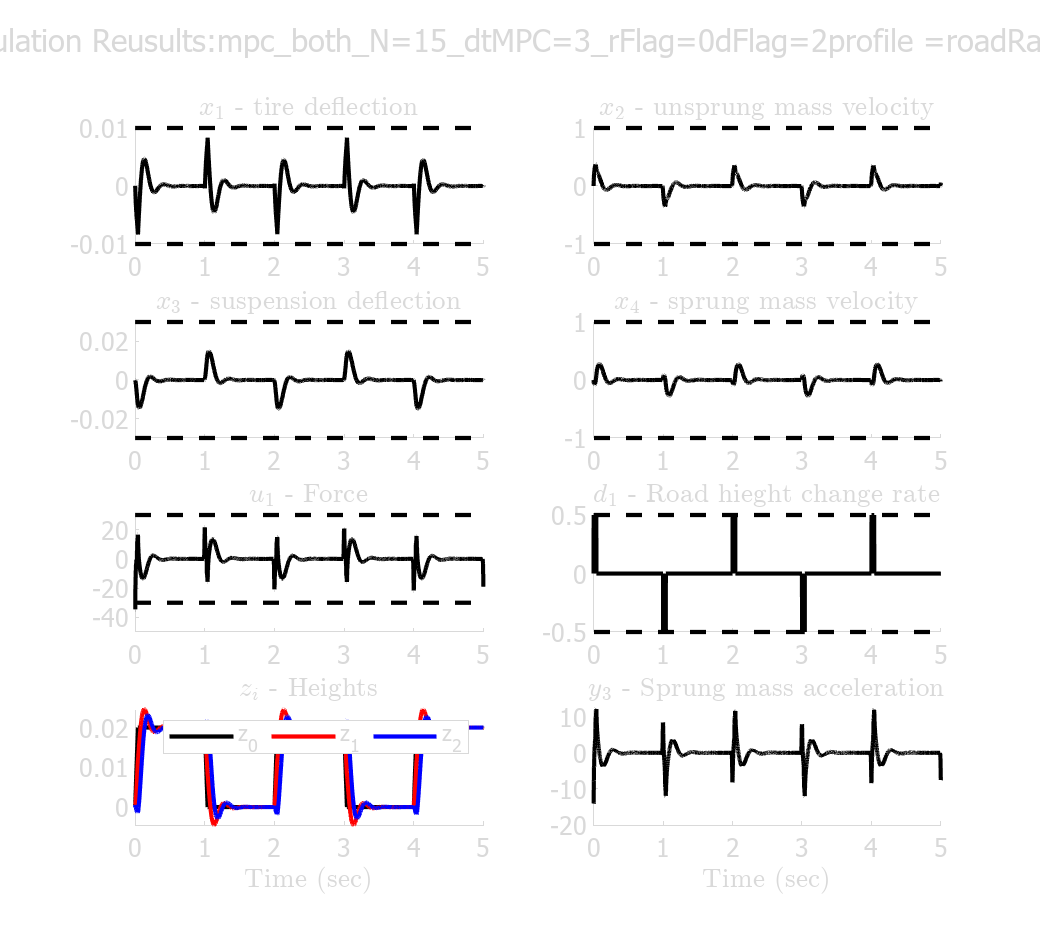
\includegraphics[width = 0.49 \columnwidth]{figs/results_mpc_both_N=15_dtMPC=3_rFlag=0_dFlag=2_roadRamps.png}
    % 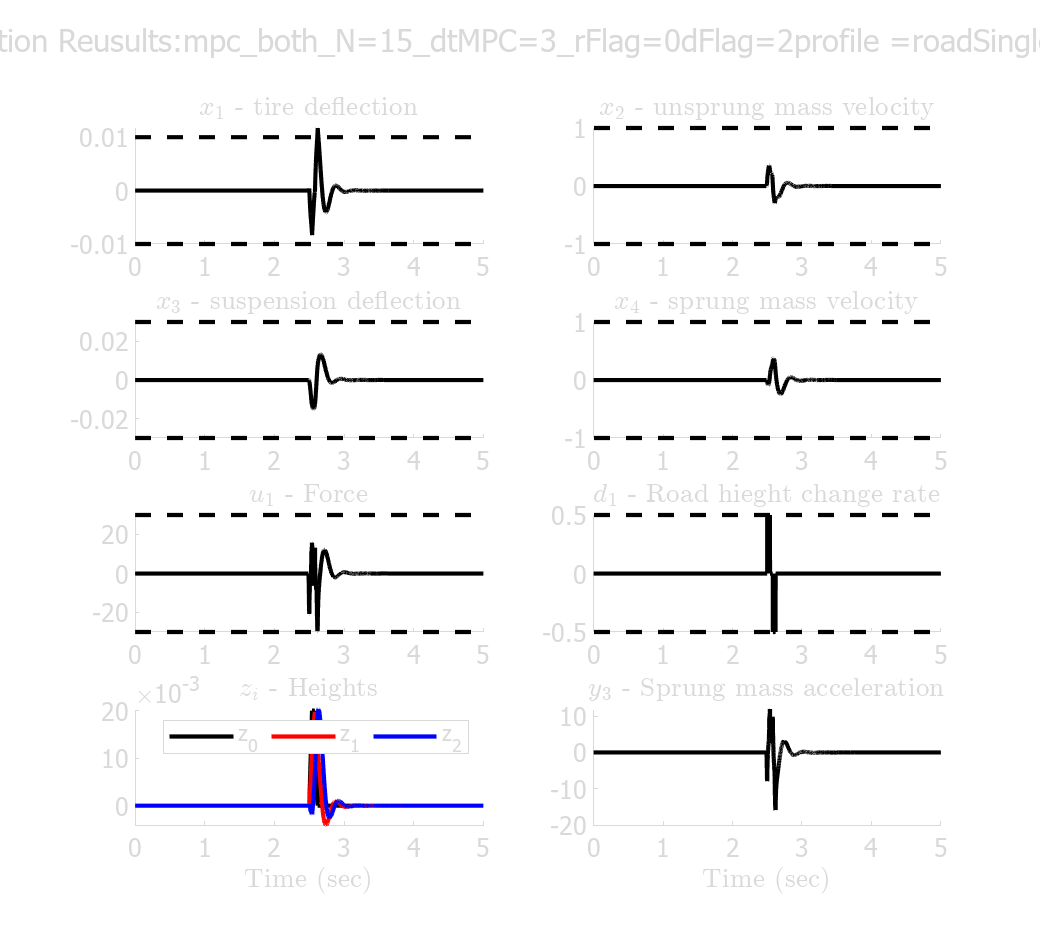
\includegraphics[width = 0.49 \columnwidth]{figs/results_mpc_both_N=15_dtMPC=3_rFlag=0_dFlag=2_roadSingleBump.png}
    \caption{Closed-loop dynamics with full disturbance information for standard MPC using $Q_both$ and $R$ updating every 3 time-steps with $N=15$ for the IRI\_737b and roadBumpHole road profiles.} \label{fig:mpc_N15_dt3_d2_r0}
\end{figure}

\newpage
% -----------------------------------------------------
% Robust MPC Controller Formulation
% -----------------------------------------------------
\section{Robust MPC Controller Formulation}
The biggest issue with all of the previous implementations has been that the bounds (specifically the tire deflection and input; and even more-so when no disturbance information is known).
In order to address this, additional constraints can be implimented to fix this.

A naive approach (something I have done prior to taking this course) is to directly attach these as hard constraints in the optimization problem (see appendix... well really the associated ones in the folder on my github) for these results; but essentially this causes an abundance of feasibility issues.

To fix this issue (something I did do prior to taking this class) would be to use those constraints instead as what I referred to as ``soft'' constraints within the objective function.
This was also tested, although disregarded, since we had already learned better solutions (namely the constraint tightening and tube MPC approaches).

Although I intuitively understand the constraint tightening approach more, the coding/implementation for the RPI sets is simpler\footnote{not a great reason, but it's why I made the choice I did}, thus this was implemented.














\end{document}
